\documentclass[11pt]{article}
\usepackage[T1]{fontenc}
\usepackage[utf8]{inputenc}
\usepackage{lmodern}
\usepackage[margin=1.05in]{geometry}
\usepackage{amsmath,amssymb,amsthm,mathtools}
\usepackage{microtype}
\usepackage{tikz}
\usetikzlibrary{arrows.meta,calc,positioning,decorations.pathreplacing}
\usepackage{enumerate,booktabs}
\usepackage{xcolor}
\definecolor{linkblue}{RGB}{30,63,103}
\usepackage[colorlinks=true,linkcolor=linkblue,citecolor=linkblue,urlcolor=linkblue]{hyperref}
\usepackage{bookmark}
\hypersetup{pdftitle={Frobenius Structures on Tame Hecke Eigensheaves},pdfauthor={OpenAI}}
\numberwithin{equation}{section}
\newtheorem{theorem}{Theorem}[section]
\newtheorem{proposition}[theorem]{Proposition}
\newtheorem{lemma}[theorem]{Lemma}
\newtheorem{corollary}[theorem]{Corollary}
\theoremstyle{definition}
\newtheorem{definition}[theorem]{Definition}
\theoremstyle{remark}
\newtheorem{remark}[theorem]{Remark}
\newcommand{\E}{\overline{\mathbb Q}_{\ell}}
\newcommand{\F}{\mathbb F}
\newcommand{\Q}{\mathbb Q}
\newcommand{\Z}{\mathbb Z}
\newcommand{\C}{\mathbb C}
\newcommand{\Gd}{\check G}
\newcommand{\Bun}{\operatorname{Bun}}
\newcommand{\Hecke}{\mathsf H}
\newcommand{\Rep}{\operatorname{Rep}}
\newcommand{\QCoh}{\operatorname{QCoh}}
\newcommand{\IndCoh}{\operatorname{IndCoh}}
\newcommand{\Loc}{\operatorname{LocSys}}
\renewcommand{\SS}{\operatorname{SS}}
\newcommand{\Nilp}{\mathrm{Nilp}}
\newcommand{\Frob}{\operatorname{Frob}}
\newcommand{\ad}{\operatorname{ad}}
\newcommand{\Ad}{\operatorname{Ad}}
\newcommand{\Spec}{\operatorname{Spec}}
\newcommand{\IC}{\operatorname{IC}}
\newcommand{\Gr}{\operatorname{Gr}}
\newcommand{\GL}{\mathrm{GL}}
\newcommand{\SL}{\mathrm{SL}}
\newcommand{\PGL}{\mathrm{PGL}}
\newcommand{\Dbar}{\overline D}
\newcommand{\lcc}{\mathrm{lcc}}
\newcommand{\id}{\mathrm{id}}
\newcommand{\RHom}{R\operatorname{Hom}}
\newcommand{\RGamma}{R\Gamma}
\newcommand{\Shv}{\operatorname{Shv}}
\newcommand{\Aut}{\operatorname{Aut}}
\newcommand{\Hom}{\operatorname{Hom}}
\newcommand{\End}{\operatorname{End}}
\newcommand{\Frac}{\operatorname{Frac}}
\newcommand{\bigboxtimes}{\mathop{\boxtimes}}
\newcommand{\mathscr}{\mathcal}
\setlength{\emergencystretch}{2em}
\title{Frobenius Structures on Tame Hecke Eigensheaves}
\author{OpenAI}
\date{October 5, 2026}
\begin{document}
\maketitle
\begin{abstract}
We construct nonzero perverse Weil Hecke eigensheaves for $\SL_n$ with Borel
level at one marked point, after a finite extension of the field of constants.
The parameter is a geometrically dense arithmetic $\PGL_n$-local system with
tame regular-unipotent monodromy on a once-punctured curve of genus at least
two over a finite field of characteristic $p>n$. The full multi-leg
eigenstructure is Frobenius compatible with the prescribed arithmetic
eigenvalue, and the geometric sheaf has parabolic nilpotent singular support.
\end{abstract}
\begingroup
\small
\tableofcontents
\endgroup
\clearpage
\section{Introduction}\label{sec:introduction}

A Hecke eigensheaf realizes a local system on a curve by the geometry of
modifications of bundles. Over a finite field, an arithmetic local system
contains more information than its geometric restriction: it also specifies
Frobenius. The corresponding automorphic object must therefore carry a
Frobenius structure that preserves its eigenisomorphisms. We construct such
objects with Borel level and tame regular-unipotent monodromy, after a finite
extension of the field of constants.

\subsection{The result}

For a smooth projective pointed curve $(X,x)$, let $G=\SL_n$ and
let $B$ be its upper-triangular Borel. The stack
$\Bun_{G,B,x}(X)$ parametrizes $G$-bundles on $X$ with a $B$-reduction
at $x$. A sheaf on this stack is locally constructible perverse if its
pullback to each smooth finite-type scheme chart, shifted by the relative
dimension of that chart, is bounded constructible and perverse. Its
parabolic global nilpotent cone $\Lambda_{\mathrm{par}}$ consists of
generically nilpotent Higgs fields with at most a simple pole at $x$ and
residue in the nilradical of the chosen Borel. Singular support is
interpreted on the same smooth charts.

For representations $\boldsymbol V=(V_i)_{i\in I}$ of the dual group
$\PGL_n$, write $\Hecke_{I,\boldsymbol V}$ for the Hecke functor with
legs in $(X\setminus\{x\})^I$. We use the relative Satake normalization
of Section~\ref{sec:conventions}, with no moving-leg shift. In particular,
the tensor-unit functor is exterior product with the constant
$\E$-sheaf on $(X\setminus\{x\})^I$.

A Weil structure over $\F_{q^m}$ means an isomorphism between the
$q^m$-Frobenius pullback of the geometric sheaf and the sheaf itself.
We require the eigenisomorphisms to respect this structure and the
Frobenius structure on the parameter.

\begin{theorem}\label{thm:main}
Let $n\geq2$, let $\F_q$ have characteristic $p>n$, let $\ell\ne p$,
and put $E=\E$. Let $X_0/\F_q$ be a smooth projective geometrically
connected curve of genus at least two, with $x_0\in X_0(\F_q)$, and
put $U_0=X_0\setminus\{x_0\}$. Suppose
\[
 \rho:\pi_1^{\mathrm{et}}(U_0)\longrightarrow\PGL_n(L)
\]
is continuous for a finite extension $L/\Q_\ell$, its geometric
restriction is Zariski dense, and its inertia at $x_0$ kills wild inertia
and has the form
\begin{equation}\label{eq:regular-monodromy}
 \rho(\gamma)=\exp\bigl(t_\ell(\gamma)N\bigr)
\end{equation}
for a regular nilpotent $N$. Here a choice of compatible
$\ell$-power roots of unity identifies the tame quotient
$\Z_\ell(1)$ with $\Z_\ell$ and defines $t_\ell$.

There are an integer $m\geq1$ and a nonzero $E$-adic Weil sheaf $M_0$ on
\[
 \Bun_{\SL_n,B,x_0}(X_0)_{\F_{q^m}}
\]
whose geometric pullback $M$ is locally constructible perverse and has
singular support in $\Lambda_{\mathrm{par}}$. If $\rho_m$ denotes the
restriction of $\rho$ to $\pi_1^{\mathrm{et}}(U_{0,\F_{q^m}})$, then
for every finite set $I$ and every family
$V_i\in\Rep_E(\PGL_n)$ there are isomorphisms of Weil sheaves
\begin{equation}\label{eq:main-eigenmaps}
 \Hecke_{I,\boldsymbol V}(M_0)
   \simeq M_0\boxtimes\bigboxtimes_{i\in I}(V_i)_{\rho_m}.
\end{equation}
They are natural in the representations and coherent for the unit,
convolution, permutations, and all fusion diagonals.
\end{theorem}

Write $k=\overline{\F}_q$, $X=X_0\times_{\F_q}k$, $x=(x_0)_k$, and
$U=U_0\times_{\F_q}k$ for the geometric curve and its punctured complement.
The Frobenius structure is required on the entire eigenstructure, rather
than only on the underlying perverse sheaf. The finite extension in the
theorem arises when a point on an auxiliary bundle stack is made invariant
under a power of Frobenius. We use Weil structures, so a compatible action
of the infinite cyclic group is sufficient.

\subsection{Background and the geometric input}

The geometric Langlands program replaces automorphic functions by sheaves
on moduli stacks of bundles and asks that Hecke eigenvalues be realized as
local systems on a curve. Drinfeld's rank-two work and Laumon's geometric
formulation established central parts of this perspective
\cite{Drinfeld,Laumon}. Frenkel, Gaitsgory, and Vilonen constructed
unramified $\GL_n$ eigensheaves, including the finite-field Weil setting;
Gaitsgory subsequently gave a geometric proof of the vanishing theorem
underlying that construction \cite{FGV,GaitsgoryVanishing}. Thus the
arithmetic compatibility of an eigenstructure is a classical requirement,
not a new condition introduced here.

For general groups, the restricted spectral stack and its action on
automorphic sheaves with nilpotent singular support were developed by
Arinkin, Gaitsgory, Kazhdan, Raskin, Rozenblyum, and Varshavsky
\cite{AGKRRV}. Gaitsgory and Raskin prove the restricted geometric
Langlands equivalence in characteristic zero and construct its
positive-characteristic specialization; in positive characteristic their
general-group result concerns a union of spectral components
\cite{GR}. We use the characteristic-zero equivalence and the spectral
action, with their precise scopes, in Section~\ref{sec:unramified}.

Our geometric input is the companion manuscript
\emph{Constructible tame Hecke eigensheaves in positive characteristic}
\cite{CT}. It constructs geometric, locally constructible perverse
eigensheaves with Borel level, parabolic nilpotent singular support, and
the full fusion-compatible eigenstructure. Its method first creates level
structure by a characteristic-zero degeneration to a separating node and
then specializes to positive characteristic. We use its nearby-cycle,
nonvanishing, perverse-truncation, and enhancement-descent theorems, stated
at their uses below. Those results do not supply Frobenius descent.
The present paper proves the additional arithmetic compatibility for
$\SL_n$ under the hypotheses of Theorem~\ref{thm:main}.

In characteristic-zero de Rham sheaf theory, F\ae rgeman constructs
coherent tame eigenobjects for irreducible regular-singular parameters,
conditional on the spectral-action and localization-compatibility inputs
specified in \cite[Sections~1.3.6--1.4.3]{Faergeman}. Regular holonomicity
and generic perversity in the tame setting remain expectations in that
preprint \cite[Remark~1.4.1.2]{Faergeman}. Our theorem establishes
perversity in the geometric $\ell$-adic setting and equips the
eigenstructure with a finite-field Weil action, for the dense parameters
with regular-unipotent boundary monodromy specified above.

The nodal geometry is part of the automorphic gluing framework of Nadler
and Yun \cite{NYAutomorphicGluing}, with twisted curves as in
Abramovich--Vistoli and Olsson \cite{AbramovichVistoli,OlssonTwisted}.
Root stacks and proper henselian invariance
of finite covers allow us to retain finite-quotient monodromy through the
two degenerations \cite{LieblichOlsson,Rydh}. The sheaf-theoretic
specialization used here is geometric nearby cycles, in the form developed
by Hansen--Scholze and Gaitsgory--Raskin and adapted to level structure
in \cite{CT,HansenScholze,GR}.

\subsection{The arithmetic constructions and the proof}

There are two extra difficulties in making the geometric construction
equivariant. First, an invariant parameter need not make an arbitrarily
chosen geometric eigenobject visibly invariant. Second, the two boundary
parameters at a separating node must be glued by a conjugation that
preserves both Frobenius and compact image.

Section~\ref{sec:unramified} treats the first difficulty. For a dense
unramified $\PGL_n$-parameter in characteristic zero, the relevant
restricted spectral component is a smooth formal space with one point.
Transport of the spectral action preserves that component. The inverse
image of its skyscraper has scalar endomorphisms and no negative
self-extensions; these properties recognize its transport up to shift.
An invariant polarization on the curve rules out a nonzero shift on the
automorphic side, giving a generator isomorphism on this particular
eigenobject. Density and the
trivial center of $\PGL_n$ force compatibility with its full eigenstructure.
This recognition argument avoids choosing an equivariant normalization
of the Langlands equivalence itself.

Section~\ref{sec:parameters} first lifts the original arithmetic parameter
to a punctured curve $C_1$ in characteristic zero. At its puncture the
Frobenius matrix $A$ and the regular nilpotent logarithm $N_1$ satisfy
$\Ad(A)N_1=qN_1$. A cocharacter commuting with $A$ scales $N_1$.
We choose a ramified cover $C_2\to C_1$ whose degree makes the required
gluing conjugator lie in a fixed compact open subgroup. The resulting
boundary identification commutes with $A$. This compact equivariant gluing
is the second reusable ingredient: inverse boundary monodromies alone
would not ensure a continuous compact-valued parameter on the smoothing.

The compatible finite torsor towers on the two punctured components glue
on balanced twisted nodal models and lift to a dense unramified parameter
on their smooth generic curve. Apply the equivariant unramified result
there. In Section~\ref{sec:nodal}, nearby cycles on a prescribed node type,
restriction to one component, and descent from enhanced to ordinary flags
produce an equivariant perverse eigensheaf on $C_1$. The restriction uses
a point defined over a finite extension of the characteristic-zero base;
a power of the generator fixes that point. Finally,
Section~\ref{sec:final} specializes this eigensheaf to the original
finite-field curve. Both specializations use a separate support-closure
argument to prove nonvanishing. Naturality of the comparisons in
Section~\ref{sec:conventions} carries the entire eigenstructure through
these steps.

\section{Equivariant Hecke systems and specialization}\label{sec:conventions}

We fix the sheaf conventions and explain which parts of the geometric
specialization formalism carry a semilinear action. The issue is compatibility
of the entire Hecke system, including collisions of moving points.

\subsection{Sheaves, level structures, and moving legs}

Write $E=\E$, $G=\SL_n$, and $\Gd=\PGL_n$, with the split forms understood
over every base field. On a smooth stack $\mathcal B$ locally of finite type,
$D_{\lcc}(\mathcal B,E)$ denotes the category of geometric adic complexes
whose pullback to each smooth finite-type scheme chart is bounded and
constructible. The bounds may depend on the chart. A complex $F$ is perverse
if $b^*F[d]$ is perverse for every smooth chart $b:Y\to\mathcal B$ of
constant relative dimension $d$. These conventions agree with
\cite[Section~2.1]{CT}.

For a pointed smooth projective curve $(X,x)$, put
\[
 \mathcal A=\Bun_{G,B,x}(X),\qquad
 \mathcal A^+=\Bun_{G,R_u(B),x}(X),\qquad T=B/R_u(B).
\]
An enhanced flag is a reduction to $R_u(B)$; forgetting the enhancement is
a representable $T$-torsor $\mathcal A^+\to\mathcal A$.
At ordinary Borel level, the trace form identifies a cotangent vector with
a Higgs field
\[
 \theta\in H^0\bigl(X,\ad(P)\otimes\omega_X(x)\bigr),
 \qquad \operatorname{Res}_x\theta\in\operatorname{Lie}R_u(B_P),
\]
where $B_P$ is the chosen Borel in the fiber at $x$. The cone
$\Lambda_{\mathrm{par}}$ consists of those fields that are nilpotent over
the function field of $X$. On a smooth chart, singular support means the
geometric adic singular support of the pulled-back complex, contained in
the smooth cotangent pullback of this cone; see
\cite[Section~3.1]{CT} and \cite{Beilinson,Barrett}.

Let $U$ be the locus of allowed modifications, disjoint from the level
point. For a finite set $I$, the Hecke stack $\mathcal H_I$ has an input
bundle map $p_I$ and an output-and-leg map
$o_I:\mathcal H_I\to\mathcal B\times U^I$.
If $\boldsymbol V=(V_i)_{i\in I}$ are representations of $\Gd$, define
\begin{equation}\label{eq:hecke-normalization}
 \Hecke_{I,\boldsymbol V}(F)
  =o_{I,*}\bigl(F\,\widetilde\boxtimes\,
                      \operatorname{Sat}_I(\boldsymbol V)\bigr).
\end{equation}
The twisted product is ordinary exterior product in input frames, descended
using equivariance of the Satake kernel. All pushforwards are taken on
finite Schubert bounds, where the output maps are proper. On a fixed-point
Schubert orbit of dimension $d_\lambda=\langle2\rho_G,\lambda\rangle$,
the simple kernel is normalized by
\begin{equation}\label{eq:satake-normalization}
 \IC_\lambda|_{\Gr^\lambda}=E[d_\lambda](d_\lambda/2).
\end{equation}
Here $\rho_G$ is the half-sum of positive roots. Since the cocharacter
lattice of $G$ is its coroot lattice, $d_\lambda$ is even. In particular
all twists in \eqref{eq:satake-normalization} are integral.
There is no moving-leg shift in \eqref{eq:hecke-normalization}.
We use geometric Satake with its fusion tensor structure \cite{MV}.

For a surjection $a:I\twoheadrightarrow J$, let
$\delta_a:U^J\to U^I$ be the collision diagonal and set
$W_j=\bigotimes_{i\in a^{-1}(j)}V_i$. The relative fusion convention is
\begin{equation}\label{eq:fusion-convention}
 (1\times\delta_a)^*\Hecke_{I,\boldsymbol V}(F)
   \simeq\Hecke_{J,\boldsymbol W}(F).
\end{equation}
This is ordinary pullback, without a codimension shift.

\begin{definition}\label{def:eigenstructure}
For a $\Gd$-local system $\vartheta$ on $U$, a coherent Hecke
eigenstructure on $F$ consists of isomorphisms
\begin{equation}\label{eq:eigenstructure}
 \Hecke_{I,\boldsymbol V}(F)
   \simeq F\boxtimes\bigboxtimes_{i\in I}(V_i)_\vartheta
\end{equation}
for all finite $I$, natural in the representations, and compatible with
the unit, successive modifications and convolution, permutations, and
all collision maps \eqref{eq:fusion-convention}, including their iterated
compatibilities. The notation $(V)_\vartheta$ means the lisse sheaf
obtained by evaluating the representation $V$ on $\vartheta$.
\end{definition}

Let $\sigma$ be a semilinear automorphism of the ground field and the curve,
preserving the split group and the level data. An equivariant sheaf has an
isomorphism $\sigma^*F\simeq F$; an equivariant eigenstructure requires
\eqref{eq:eigenstructure} to commute with this isomorphism and the specified
isomorphism $\sigma^*\vartheta\simeq\vartheta$. We use the group generated
by $\sigma$, so the one isomorphism determines all its iterates and inverses.
Transport acts on the base, not on the coefficient field $E$.
At a finite-field fiber the ground-field action $a\mapsto a^q$ gives the
arithmetic convention. Inverting the generator everywhere gives the usual
geometric Frobenius convention for Weil sheaves.

\subsection{Satake transport and its Weil normalization}

\begin{lemma}\label{lem:satake-transport}
Semilinear isomorphisms of pointed curves identify the relative Satake and
Hecke systems, compatibly with all the operations in
Definition~\ref{def:eigenstructure}. In representation labels the required
symmetric tensor comparison is unique. The same assertion holds for
extension between algebraically closed characteristic-zero fields.
\end{lemma}

\begin{proof}
Transport preserves the split Schubert orbits, their intersection complexes,
convolution diagrams, and fusion diagrams. Thus it gives a symmetric tensor
equivalence of the spherical Satake categories preserving all highest-weight
labels. Under Satake it is a symmetric tensor autoequivalence of
$\Rep_E(\PGL_n)$ with trivial outer automorphism. Over the algebraically
closed coefficient field it is tensor isomorphic to the identity: the
fiber-functor torsor is trivial and the remaining group automorphism is inner.
Two such isomorphisms differ by a tensor automorphism of the identity functor,
namely an element of $Z(\PGL_n)$, which is trivial.

Use this comparison for the full geometric system. On separated legs it is
the exterior product comparison. The fusion extensions, proper convolution
maps, and their exchange transformations are transported together, so their
compatibility maps agree. In the kernel categories the fusion extensions
are middle extensions with the usual perverse leg shifts; a comparison on
the separated locus determines them. Applying the corresponding natural
sheaf operations gives the Hecke comparison. Algebraically closed base
extension has the same properties: it preserves the simple kernels and
convolution and is an equivalence on spherical Satake. Uniqueness again
identifies its representation labels.
\end{proof}

\begin{lemma}\label{lem:normalized-weil-satake}
Over a finite field, the split Weil structures on
\eqref{eq:satake-normalization} give a symmetric tensor Satake system,
with ordinary coefficient multiplicity spaces carrying trivial action.
Its Frobenius comparison is the one in
Lemma~\ref{lem:satake-transport}.
\end{lemma}

\begin{proof}
We verify the normalization, since purity alone would not specify the
Frobenius scalars. Resolve a split affine Schubert variety by its
Bott--Samelson resolution, using the Iwahori stratification. Its iterated
projective-line-bundle structure is defined over the finite field. The
projective-bundle formula gives scalar geometric Frobenius $q^j$ on
$H^{2j}$ and zero odd cohomology. After the shift and twist
$[d_\lambda](d_\lambda/2)$, the scalar on degree $i$ is $q^{i/2}$.

In perverse degree zero of the proper direct image, the full-support
intersection complex occurs with multiplicity one. The decomposition
theorem \cite[Theorems~5.3.8 and~5.4.5]{BBD} makes its isotypic summand geometrically well defined and hence
Frobenius stable, with the normalization fixed on the open orbit. The
Frobenius-stable perverse Leray filtration, whose spectral sequence
degenerates by the same theorem, exhibits each cohomology group of this
summand as a subquotient of the corresponding scalar cohomology group.
Thus
\[
 H^i(\Gr,\IC_\lambda)\text{ has Frobenius as on }E(-i/2)
 \quad(i\text{ even}),\qquad H^i=0\quad(i\text{ odd}).
\]

The cohomological convolution comparison is graded and Frobenius
compatible. Indeed it is constructed by K\"unneth on separated legs and
fusion over the split affine line
\cite[Lemma~6.1, Equations~(6.2a)--(6.2c), and Section~14]{MV}.
The cohomology system is lisse across
collisions and geometrically constant: it is constant on the separated
locus in the coordinate trivializations, and lisseness extends this
constancy. Comparison between rational configurations therefore commutes
with Frobenius; binary tensor comparison uses the rational configurations
$(0,1)$ and $(0,0)$, available over every finite field.
The scalar rule is consequently the same for convolution
and the corresponding tensor product. Every graded tensor comparison on
total cohomology commutes with these scalars. Faithfulness of the
cohomological Satake fiber functor shows that the kernel tensor maps do
as well. In particular, the induced Frobenius action on the geometric
multiplicity space $\Hom(\IC_\nu,\IC_\lambda*\IC_\mu)$ is trivial:
source and target cohomology have the same scalar in each degree,
and the cohomological fiber functor is faithful.
Fusion extends the compatibility to the relative system.
Finally, the uniqueness in Lemma~\ref{lem:satake-transport} identifies
this Weil comparison with the transport comparison.
\end{proof}

\subsection{The specialization input with an action}

The geometric result we need is stronger than one-point Hecke commutation.
It is the combination of Propositions~2.1 and~5.1 of \cite{CT}, with
the following relative setup. Let $S=\Spec R$ be an excellent complete
strictly henselian discrete valuation trait with algebraically closed
residue field and with $\ell$ invertible. Fix a geometric generic point
$\bar\eta$ and write $s$ for the closed point. Let $\mathcal B/S$ be a
smooth locally finite-type bundle stack and let $U/S$ be a smooth scheme
of relative dimension one of allowed legs. Bounded Hecke correspondences
have proper representable output maps, and in coordinates and input frames
they have the split Schubert local models with their spherical kernels.
The setup includes ordinary and enhanced level disjoint from the legs,
and the twisted nodal families used below.

\begin{proposition}[Geometric specialization and transport]
\label{prop:equivariant-specialization}
In this setup, geometric nearby cycles preserve local bounded
constructibility and are perverse exact. They admit natural isomorphisms
\begin{equation}\label{eq:hecke-specialization}
 \Hecke^s_{I,\boldsymbol V}(\Psi F)
  \xrightarrow{\ \sim\ }
  \Psi\bigl(\Hecke^{\bar\eta}_{I,\boldsymbol V}(F)\bigr)
\end{equation}
compatible with the unit, convolution, permutations, and every fusion
diagonal. Suppose $F$ has a coherent eigenstructure with parameter
$\vartheta_{\bar\eta}$. For each representation, suppose its evaluation
sheaf has a lisse lattice whose finite reductions extend lisse after
finite trait extensions, compatibly on further extensions and with the
reductions of a special-fiber tensor system $\vartheta_s$. Then $\Psi F$
has a coherent eigenstructure with eigenvalue $\vartheta_s$.

If the models, $F$ with its given coherent eigenstructure, and these
tensor-specialization data carry a semilinear generator, with a
compatible lift to $\bar\eta$, all the
comparisons and the resulting eigenstructure are equivariant. For the
finite-stage lattice models one may use compatible invariant trait
extensions. No single finite extension is required for all reductions.
\end{proposition}

\begin{proof}
The geometric assertions are exactly
\cite[Propositions~2.1 and~5.1]{CT}; the foundational nearby-cycle
formalism is also described in \cite[Section~4.1]{GR} and
\cite[Theorems~4.1 and~6.7]{HansenScholze}. In particular, these are
geometric nearby cycles without inertia invariants, and the input need
not descend over one finite extension of the fraction field.

We explain the additional equivariance. An isomorphism of traits and
models, together with its lift to the geometric generic point, identifies
the defining nearby-cycle diagrams. The pullback, proper-pushforward,
and tensor exchange maps therefore commute with its transport. In input
frames the Hecke comparison is the natural exterior-product exchange
with a Satake kernel, followed by proper-pushforward exchange. This is
the construction in \cite[Section~5]{CT}, including its comparison on
collision diagonals. The Satake-label identification in
\cite[Lemma~5.3]{CT} also commutes with transport: the two composites
are tensor comparisons and hence agree by
Lemma~\ref{lem:satake-transport}.

On the eigenvalue side, the lisse tensor comparison is natural at every
finite lattice reduction and every further trait extension. Passing to
the adic system preserves this naturality. Thus
\eqref{eq:hecke-specialization} transports the equivariant eigenmaps
and all their diagrams. The convolution and nested diagonal identities
are identities of the same exchange transformations; they require no
separate choices. At a finite-field fiber their Satake structures are
the normalized Weil structures by
Lemma~\ref{lem:normalized-weil-satake}.
\end{proof}

\subsection{The characteristic restriction for \texorpdfstring{$\SL_n$}{SLn}}

The remaining geometric inputs of \cite{CT} have four Lie-theoretic
hypotheses: a nondegenerate invariant symmetric form, also nondegenerate
on every Levi's Lie-algebra center; Chevalley restriction for every Levi;
scheme-theoretic semisimple centralizers that are Levis; and containment
of every nilpotent element, over every field extension, in the nilradical
of a parabolic defined over that field. We verify them to make the
characteristic restriction in the main theorem explicit.

\begin{lemma}\label{lem:lie-hypotheses}
For $G=\SL_n$ over an algebraically closed field of characteristic zero or of characteristic
$p>n$, the hypotheses H1--H4 of \cite[Theorem~1.1]{CT} hold.
\end{lemma}

\begin{proof}
The invariant form $\kappa(X,Y)=\operatorname{tr}(XY)$ is nondegenerate
on $\mathfrak{sl}_n$, since $n$ is invertible. For a block Levi with
block sizes $n_1,\ldots,n_r$, its restriction to the Lie-algebra center
is the diagonal form with entries $n_i$ on
\[
 \{(z_i):\textstyle\sum_i n_i z_i=0\}.
\]
This hyperplane is the orthogonal complement of $(1,\ldots,1)$,
whose squared length is $n$. All $n_i$ and $n$ are invertible, so the
restricted form is nondegenerate.

Chevalley restriction for these Levis follows by block diagonalization
on the dense regular-semisimple locus. Block-symmetric polynomials in
the eigenvalues lift by the block characteristic polynomials.
The Weyl-group order divides $n!$, which is invertible; averaging shows
that invariants on the total-trace-zero hyperplane are restrictions of
invariants on the full diagonal space. Block diagonalization may be
performed in the determinant-one Levi, by adjusting the determinant
with an element of the diagonal centralizer.

The scheme-theoretic centralizer of a semisimple Lie-algebra element
is its block Levi, as follows directly from the matrix commutation
equations. Finally, over every field extension, vanishing of the
positive-degree invariant polynomials says that the matrix is nilpotent.
A basis adapted to its kernel filtration puts it in a strictly triangular
Lie algebra defined over that field. It therefore lies in the
nilradical of a rational Borel, which supplies the required rational
parabolic.
\end{proof}

\section{An equivariant unramified eigencomplex}\label{sec:unramified}

The first specialization will start with an unramified eigencomplex on a
smooth projective curve in characteristic zero.  The geometric existence
theorem supplies such a complex, but does not by itself supply the
semilinear action needed here.  We obtain that action by using the
particular eigencomplex attached to a spectral skyscraper.  Its spectral
component is preserved by transport, and the skyscraper can be recognized
from its endomorphisms.  A second rigidity argument then shows that every
isomorphism with its transport respects the full eigenstructure.

\begin{proposition}\label{prop:equivariant-unramified}
Let $C$ be a smooth projective connected curve of genus at least two over
an algebraically closed field $K$ of characteristic zero.  Let $f$ be a
semilinear automorphism of $C$ with an ample line bundle $\mathcal L$
and an isomorphism $f^*\mathcal L\simeq\mathcal L$.  Let $G=\SL_n$
and $\Gd=\PGL_n$.  Suppose that $\tau$ is a continuous $\Gd$-local system
on $C$, defined over a finite extension of $\Q_\ell$, with Zariski-dense
image and an isomorphism $u:f^*\tau\xrightarrow{\sim}\tau$.

There is a nonzero locally bounded constructible complex $D_\tau$ on
$\Bun_G(C)$, with nilpotent singular support, a full coherent Hecke
eigenstructure of eigenvalue $\tau$, and an isomorphism
\[
                 b:f^*D_\tau\xrightarrow{\sim}D_\tau
\]
compatible with that eigenstructure and $u$.  The object $D_\tau$ is compact
in the automorphic nilpotent category.  The eigenstructure uses the
relative Satake normalization of Section~\ref{sec:conventions} and is
compatible with unit, convolution, permutations, and every fusion
diagonal.  The isomorphisms $b$ and $u$ define compatible actions of
$\Z$ on the eigencomplex and its eigenvalue.
\end{proposition}

Here $f^*$ denotes transport on the curve and on its bundle stack, with
the coefficient field $\E$ fixed.  We prove the proposition in three
steps: identify the spectral summand and its behavior under transport,
recognize the transported object without a shift, and prove uniqueness
of the coherent eigenstructure on that object.

\subsection{The spectral skyscraper and transport of the action}

Write
\[
 \mathcal S=\Loc_{\Gd}^{\mathrm{restr}}(C),\qquad
 \mathcal D_C=\Shv_{\Nilp}(\Bun_G(C)).
\]
The first stack parametrizes local systems with restricted variation;
the second is the full automorphic category with global nilpotent
singular support.  We use the following precise characteristic-zero
input from the proof of \cite[Lemma~8.1]{CT}.  The Gaitsgory--Raskin
equivalence
\begin{equation}\label{eq:unramified-equivalence}
 \mathcal D_C\simeq\IndCoh_{\Nilp}(\mathcal S)
\end{equation}
is linear for the $\QCoh(\mathcal S)$-action, and the inclusion of
$\mathcal D_C$ in the ambient automorphic category preserves compact
objects \cite[Main Theorem~1.3.9(ii), Lemma~1.3.7, and Theorem~1.1.7]{GR}.
These statements apply to geometric $\E$-adic sheaves over an arbitrary
algebraically closed characteristic-zero field
\cite[Section~2.3]{GR}.  The spectral action agrees, through universal
evaluation, with the coherent Hecke action
\cite[Main Theorem~14.3.2 and Section~14.3.3]{AGKRRV}.
As in \cite[Lemma~8.1]{CT}, we identify the external Satake labels with
our input--output convention: if a tensor relabeling $\alpha$ is required,
the external point is $\tau\circ\alpha^{-1}$.  Evaluation at the point
denoted by $\tau$ below is therefore exactly $V\mapsto V_\tau$.

Let $i_\tau:\Spec\E\to\mathcal S$ denote this point, and put
\[
       \delta_\tau=i_{\tau,*}^{\IndCoh}\E.
\]
We recall the local description used in \cite[Lemma~8.1]{CT}, since it
will also recognize the transport of this object.  The components of
$\mathcal S$ are indexed by semisimple parameters; the component of an
irreducible parameter has only one isomorphism class of geometric points
\cite[Proposition~3.7.2 and Corollary~3.7.5]{AGKRRV}.  Density makes $\tau$
irreducible and gives
\begin{equation}\label{eq:unramified-centralizer}
 \Aut(\tau)=Z_{\Gd}(\operatorname{im}\tau)=Z(\Gd)=1.
\end{equation}
The tangent complex of $\mathcal S$ at $\tau$ is
$\RGamma(C,\ad(\tau))[1]$
\cite[Section~21.2.1]{AGKRRV}.  Its degree $-1$ cohomology is zero by
\eqref{eq:unramified-centralizer}.  The invariant nondegenerate form on
$\operatorname{Lie}(\Gd)$ and Poincar\'e duality give
\[
 H^2(C,\ad(\tau))
       \simeq H^0(C,\ad(\tau))^\vee(-1)=0.
\]
Thus the open-and-closed component $\mathcal S_\tau$ containing $\tau$
has no infinitesimal automorphisms or obstructions and is a smooth
one-point formal polydisc, with tangent space $H^1(C,\ad(\tau))$.

For this formal component we use the completion description
\[
 \IndCoh(\mathcal S_\tau)
       \simeq\IndCoh(\mathbb A^d_{\E})_{\{0\}},
 \qquad d=\dim_{\E} H^1(C,\ad(\tau)),
\]
as in \cite[Sections~21.1.7--21.1.10]{AGKRRV}; the right-hand category
consists of objects set-theoretically supported at the origin.  Its
compact objects are bounded coherent complexes with this support.
Indeed, coherent complexes with this support are compact and generate the supported
category; on the smooth affine space this is also the usual generation
by the Koszul complex at the origin.  In particular their cohomology
modules have finite length.  The skyscraper $\delta_\tau$ is nonzero and
compact.  Since the formal component is smooth, it has no spectral
obstruction directions, so $\delta_\tau$ has nilpotent spectral singular
support.  This is the ind-coherent singular-support condition, rather
than the microlocal support of a constructible skyscraper.

Choose an equivalence \eqref{eq:unramified-equivalence}, and let $D_\tau$
be the inverse image of $\delta_\tau$.  It is compact in $\mathcal D_C$ and
in the ambient automorphic category.  Compact automorphic objects are
bounded constructible on every finite-type smooth chart
\cite[Appendix~F, Section~F.2.2]{AGKRRV}, so $D_\tau$ is locally bounded
constructible.  Its full eigenstructure is the one constructed in
\cite[Lemma~8.1]{CT}: the module identities
\begin{equation}\label{eq:skyscraper-evaluation}
 A\otimes\delta_\tau
       \simeq i_{\tau,*}^{\IndCoh}(i_\tau^*A),
       \qquad A\in\QCoh(\mathcal S),
\end{equation}
applied to universal evaluation over $C^I$, give
\begin{equation}\label{eq:unramified-eigenmaps}
 \Hecke_{I,(V_i)}(D_\tau)
   \simeq D_\tau\boxtimes
            \Bigl(\boxtimes_{i\in I}(V_i)_\tau\Bigr).
\end{equation}
The unit, tensor, permutation, and fusion maps come from the same
universal evaluation system.  Spectral linearity transports all of them
together.  This proves the required geometric assertions about $D_\tau$.

The remaining issue is the action of $f$.  It is enough at this stage to
preserve the summand corresponding to $\mathcal S_\tau$; no equivariance
of the chosen equivalence \eqref{eq:unramified-equivalence} is required.

\begin{lemma}\label{lem:spectral-action-transport}
Semilinear transport by $f$ identifies the automorphic spectral action
with the action for the transported curve and its restricted stack of
local systems.  Consequently, if $f^*\tau\simeq\tau$, transport preserves
the summand of $\mathcal D_C$ corresponding to $\mathcal S_\tau$.
\end{lemma}

\begin{proof}
We compare the finite-set Hecke action data that characterize the
spectral action.  These data include derived representation labels,
leg factors $\operatorname{QLisse}(C)^{\otimes I}$, and their higher
compatibilities; $\operatorname{QLisse}(C)$ is the category of
quasi-lisse sheaves of \cite[Section~8.1.1]{AGKRRV}.  Exterior product
realizes the leg factors on $C^I$.  We must transport both the Hecke
diagrams and this quasi-lisse factorization.

First consider the geometric Hecke diagrams.  Transport by $f$ is
an exact $\E$-linear equivalence preserving nilpotent singular support.
It takes every Hecke correspondence over $C^I$ to its transported
correspondence and commutes with pullback, tensor product, convolution
pushforward, and their exchange maps.  Lemma~\ref{lem:satake-transport}
compares the Satake kernels and their tensor and fusion maps.
Dualizing complexes are transported as well, so the comparison also
applies when the action is expressed with dualizing pullback conventions.
The resulting comparison is one of the actual sheaf operations and
their structural maps, including the geometric maps in the leg categories.

To pass from ordinary representations to the derived labels, use the
construction of \cite[Sections~B.3.6--B.3.8]{GKRV}, recalled in
\cite[Section~14.2.2]{AGKRRV}: bounded-derived extension, restriction
to compact objects, and then ind-extension.  On the perverse
representation objects, the preceding comparison identifies the
Satake diagrams with all their structural maps.  The universal
property of the bounded derived category extends it exactly and
preserves the coherent finite-set diagrams.  The resulting right-lax
monoidal structure maps are isomorphisms.  Restriction to compact
objects and ind-extension therefore give the comparison for the
continuous derived action.  This uses the specified extension of the
representation action; it does not identify the whole derived
spherical sheaf category with the derived representation category.

It remains to compare the quasi-lisse factorization.  Transport
identifies $\operatorname{QLisse}(C)^{\otimes I}$ with the corresponding
category for the transported curve.  The exterior-product embedding
used in \cite[Section~14.2.5]{AGKRRV} is fully faithful, so the
comparison just constructed also identifies the Hecke action with
values in these leg categories.  This is the action developed in
\cite[Sections~14.2.5--14.2.8 and Main Theorem~14.3.2]{AGKRRV}.

We have now compared the full finite-set action data.  Transport also
identifies the universal evaluation objects on the restricted stacks.
By \cite[Theorem~8.1.4]{AGKRRV}, universal evaluation gives an
equivalence between the space of $\QCoh(\mathcal S)$-actions and the
space of these data, with their higher compatibilities.  Consequently
the conjugate of the spectral action under transport is the spectral
action of the transported curve.

The component $\mathcal S_\tau$ is carried to the component of
$f^*\tau$.  When these parameters are isomorphic, its component
idempotent is preserved.  This idempotent acts as the identity on
$D_\tau$, and hence also on $f^*D_\tau$, proving the final assertion.
\end{proof}

\subsection{Recognizing the transported object}

The preceding lemma places $f^*D_\tau$ in the same spectral component as
$D_\tau$.  We now recognize its image there.  The required elementary
criterion is useful independently of the spectral setting.

\begin{lemma}\label{lem:point-object}
Let $(R,\mathfrak m)$ be a commutative local $\E$-algebra with residue
field $\E$, and let $P$ be a nonzero bounded complex of $R$-modules whose
cohomology modules have finite length.  Suppose that
\[
 \Hom_{D(R)}(P,P)=\E,\qquad
 \Hom_{D(R)}(P,P[j])=0\quad(j<0).
\]
Then $P\simeq\E[r]$ for an integer $r$.
\end{lemma}

\begin{proof}
Let $a$ and $b$ be the least and greatest degrees with nonzero
cohomology.  Any two nonzero finite-length modules over $R$ admit a
nonzero map from the first to the second: take a quotient of the first
onto $\E$ and an inclusion of $\E$ into the socle of the second.  Thus,
if $a<b$, there is a nonzero map
$h:H^b(P)\to H^a(P)$.  The truncation maps give a composite
\[
 P\longrightarrow H^b(P)[-b]
   \xrightarrow{h[-b]}H^a(P)[-b]
   \longrightarrow P[a-b].
\]
Its map on degree $b$ cohomology is $h$, so it is a nonzero negative-degree
endomorphism.  This contradicts the hypothesis.  Hence $a=b$, and $P$ is
a shift of a single finite-length module $M$.

Every element of $\mathfrak m$ acts nilpotently on $M$.  Since
$\End_R(M)=\E$, this action is a nilpotent scalar and is therefore zero.
Thus $M$ is an $\E$-vector space, and all of its $\E$-linear
endomorphisms are $R$-linear.  The equality $\End_R(M)=\E$ forces
$\dim_{\E} M=1$.
\end{proof}

For the skyscraper, and therefore for $D_\tau$, we have
\begin{equation}\label{eq:unramified-endomorphisms}
 H^0\RHom(D_\tau,D_\tau)=\E,\qquad
 H^j\RHom(D_\tau,D_\tau)=0\quad(j<0).
\end{equation}
These are the ambient automorphic Hom groups, since $\mathcal D_C$ is a
full subcategory.  Transport preserves both these groups and compactness.
Lemma~\ref{lem:spectral-action-transport} places $f^*D_\tau$ in the
$\mathcal S_\tau$ summand.  Its image under
\eqref{eq:unramified-equivalence} is therefore a bounded coherent complex
supported at the origin of the smooth formal component.  Applying
Lemma~\ref{lem:point-object} to the local ring at that origin gives
\begin{equation}\label{eq:unramified-possible-shift}
                    f^*D_\tau\simeq D_\tau[r]
\end{equation}
for some $r\in\Z$.

We eliminate the shift on a bounded open, so no global cohomological
bound on $\Bun_G(C)$ is needed.  Use the $f$-invariant ample line bundle
$\mathcal L$ in the statement.
For each sufficiently large integer $m$, let
$\mathcal U_m\subset\Bun_{\SL_n}(C)$ be the open substack on which the
associated vector bundle $\mathcal V$ satisfies
\[
 \mathcal V\otimes\mathcal L^m\text{ is globally generated},
 \qquad H^1(C,\mathcal V\otimes\mathcal L^m)=0.
\]
These conditions are open and the opens cover the bundle stack by Serre
vanishing.  Each $\mathcal U_m$ is of finite type: rank and trivialized
determinant fix the Hilbert polynomial, the displayed conditions fix
$h^0$, and a choice of basis of sections gives the usual finite-type
Quot presentation.  Adding the determinant trivialization is also a
finite-type condition.  Because $f$ preserves $\mathcal L$, every
$\mathcal U_m$ is invariant under transport.

Choose $m$ with $D_\tau|_{\mathcal U_m}\ne0$.  On a finite-type smooth
atlas of $\mathcal U_m$, local bounded constructibility gives a finite
cohomological interval; descent gives the same boundedness on
$\mathcal U_m$.  Consequently
\[
 S_m=\{j\in\Z:\mathcal H^j(D_\tau|_{\mathcal U_m})\ne0\}
\]
is finite and nonempty.  Pullback along the automorphism of
$\mathcal U_m$ is exact and conservative, so it preserves $S_m$.
Equation~\eqref{eq:unramified-possible-shift} gives $S_m=S_m-r$, which
forces $r=0$.  We have obtained an isomorphism
$b:f^*D_\tau\simeq D_\tau$.  It remains to verify its compatibility with
the Hecke eigenmaps.

\subsection{Uniqueness of the full eigenstructure}

For $I$ a finite set and $L_1,L_2$ finite-rank lisse $\E$-sheaves on
$C^I$, there is a natural external-product formula
\begin{equation}\label{eq:unramified-hom-kunneth}
 \RHom(D_\tau\boxtimes L_1,D_\tau\boxtimes L_2)
 \simeq
 \RHom(D_\tau,D_\tau)\otimes_{\E}
       \RGamma(C^I,L_1^\vee\otimes L_2).
\end{equation}
We explain its applicability to the non-quasicompact bundle stack.
On every finite-type smooth scheme chart, the restrictions of $D_\tau$
are bounded constructible, and the usual constructible Hom--K\"unneth
formula applies.  Equivalently, one can use adjunction for the projection
to the chart, proper base change for $C^I$, and the projection formula.
The second factor in \eqref{eq:unramified-hom-kunneth} is a bounded
finite-dimensional $\E$-complex, hence perfect.  Tensoring with it
commutes with the limits computing smooth descent and restriction over
finite-type opens of the bundle stack.  The chartwise formulas therefore
give the displayed global formula.  On constructible chart objects these
are also the Hom complexes in the ambient ind-sheaf category.

Both factors on the right are concentrated in nonnegative degrees, by
\eqref{eq:unramified-endomorphisms} and the fact that the $L_i$ are
ordinary lisse sheaves.  Thus
\begin{align}
 \Hom(D_\tau\boxtimes L_1,D_\tau\boxtimes L_2)
       &\simeq\Hom(L_1,L_2),\label{eq:unramified-hom-zero}\\
 H^j\RHom(D_\tau\boxtimes L_1,D_\tau\boxtimes L_2)
       &=0\qquad(j<0).\label{eq:unramified-hom-negative}
\end{align}
The first identification sends a lisse-sheaf map $a$ to
$\id_{D_\tau}\boxtimes a$.

\begin{lemma}\label{lem:unramified-eigenstructure-unique}
The complex $D_\tau$ admits a unique full coherent Hecke eigenstructure
with eigenvalue $\tau$.  Consequently every isomorphism
$f^*D_\tau\simeq D_\tau$ is compatible with the eigenstructure and the
given isomorphism $u:f^*\tau\simeq\tau$.
\end{lemma}

\begin{proof}
Compare two full eigenstructures.  For each finite set $I$ and tuple of
representations $(V_i)$, their eigenmaps differ by an automorphism of
\[
       D_\tau\boxtimes\Bigl(\boxtimes_{i\in I}(V_i)_\tau\Bigr).
\]
By \eqref{eq:unramified-hom-zero}, this automorphism is uniquely
$\id_{D_\tau}\boxtimes a_{I,(V_i)}$, where $a_{I,(V_i)}$ is an
automorphism of the lisse factor.  Naturality of the eigenstructures
makes the one-leg maps $a_V$ natural in $V$.  Compatibility with
successive Hecke operations, on the locus of distinct legs, identifies
the maps $a_{I,(V_i)}$ with exterior products of the one-leg maps.
Equality on that dense open determines maps of lisse sheaves on $C^I$.
Fusion along the diagonal then gives
\[
          a_{V\otimes W}=a_V\otimes a_W,
          \qquad a_{\E}=\id.
\]
Thus the $a_V$ form a tensor automorphism of the local-system functor
$V\mapsto V_\tau$.  Its group is the centralizer of the monodromy of
$\tau$ in $\Gd$, which is trivial by
\eqref{eq:unramified-centralizer}.  All $a_V$, and hence all
$a_{I,(V_i)}$, are identities.  The two systems of eigenmaps agree.

This also proves uniqueness at the level of coherent structures.
Equation~\eqref{eq:unramified-hom-negative} says that the mapping spaces
between the displayed targets have no positive homotopy groups.
The eigenmaps identify the successive Hecke transforms in the
compatibility diagrams with targets of the same form.  Hence there is
no additional choice of higher homotopies in the unit, convolution,
permutation, or fusion compatibilities.  The resulting natural
transformation on ordinary representation labels
has a unique exact continuous extension by the universal properties of
the stable and ind constructions defining the spectral action.

Now transport the eigenstructure of $D_\tau$ by $f$, use $u$ on its
eigenvalue, and use any isomorphism $b:f^*D_\tau\simeq D_\tau$ on the
automorphic factor.  Lemma~\ref{lem:satake-transport} makes this a full
eigenstructure on $D_\tau$ with eigenvalue $\tau$.  The uniqueness just
proved identifies it with the original one, which is the claimed
compatibility of $b$.
\end{proof}

\begin{proof}[Proof of Proposition~\ref{prop:equivariant-unramified}]
The inverse image of $\delta_\tau$ constructed above is nonzero, compact,
locally bounded constructible, and carries the coherent geometric
eigenstructure \eqref{eq:unramified-eigenmaps}.  Its membership in
$\mathcal D_C$ gives nilpotent singular support.  Spectral-action transport,
Lemma~\ref{lem:point-object}, and the invariant-open argument give an
isomorphism $b:f^*D_\tau\simeq D_\tau$.
Lemma~\ref{lem:unramified-eigenstructure-unique} proves its compatibility
with $u$ and all eigenmaps.  Iterating $b$ and its inverse defines the
action of the free cyclic group, with the corresponding iterations of
$u$ on the eigenvalue.  The eigenstructure compatibilities persist under
these iterations.  This is the asserted $\Z$-equivariant eigencomplex.
\end{proof}

\section{Arithmetic towers and equivariant gluing at a node}
\label{sec:parameters}

We construct the parameter to which the unramified input of
Proposition~\ref{prop:equivariant-unramified} will be applied.  There are
two steps.  First we lift the arithmetic parameter $\rho$ to a punctured
curve in characteristic zero, retaining its Frobenius action and its
entire boundary homomorphism.  We then place this lift on one component
of a separating nodal curve and extend it to an unramified parameter on
a smooth generic fiber.  In the second step the gluing must preserve
both Frobenius and compactness of the monodromy image.  A ramified
auxiliary component will allow us to satisfy these two conditions
simultaneously.

\subsection{Lifting the arithmetic parameter}

With $k=\overline{\F}_q$, set
\begin{equation}\label{eq:coefficient-traits}
 R_0=W(\F_q),\qquad D=\Frac(R_0),\qquad
 R=W(k),\qquad K=\overline{\Frac(R)},\qquad
 \Dbar=\overline D\subset K.
\end{equation}
Here $\Dbar$ is the algebraic closure of $D$ inside $K$.  The ring $R$
is an excellent complete strictly henselian discrete valuation ring
with residue field $k$.  Extend the Witt-vector automorphism of $R$
induced by $a\mapsto a^q$ on $k$ to an automorphism $\varphi$ of $K$.
It fixes $D$ and preserves $\Dbar$.  On roots of unity of $\ell$-power
order it acts by $\zeta\mapsto\zeta^q$, as follows from their
Teichm\"uller lifts in $R$.  We use the same letter for these compatible
actions, with the coordinate orientation fixed in
Section~\ref{sec:conventions}.

Choose a smooth projective pointed lift
\[
 (\mathscr X,\mathfrak x)\longrightarrow\Spec R_0
 \quad\text{of }(X_0,x_0),
 \qquad \mathscr U=\mathscr X\setminus\mathfrak x.
\]
Pointed deformations are unobstructed because
$H^2(X_0,T_{X_0}(-x_0))=0$; an ample line bundle also lifts, and formal
algebraization gives the projective family.  This is the lifting
construction of \cite[Section~8.5]{CT}, here performed over $R_0$ so as
to retain the field of definition.  Write
\[
 (C_1,x_1)=(\mathscr X,\mathfrak x)_D,
 \qquad U_1=C_1\setminus\{x_1\}.
\]
By smoothness, a function $t$ on a neighborhood of $\mathfrak x$ over
$R_0$ may be chosen as a relative parameter.  Its differential
trivializes the conormal line of the section.  We also regard $t$ as a
rational function on $C_1$.

For an integer $d$ invertible in $R_0$, the coordinate $t$ identifies
the residual gerbe of $\mathscr X(\sqrt[d]{\mathfrak x})$ with
$B\mu_d$ over $R_0$: it trivializes the divisor line by $1/t$ and
thereby specifies its trivial $d$th root.  Pulling a finite torsor
back to this neutral object gives its boundary fiber.  A frame over
the strictly henselian base $R$ identifies that fiber with its finite
structure group, acting on itself on the right.  In this frame, both inertia
and semilinear transport are recorded by left multiplication.  The
construction below chooses such frames compatibly through the tower.

\begin{proposition}\label{prop:lifted-parameter}
The arithmetic representation $\rho$ determines a continuous
parameter
\[
 \sigma_1:\pi_1^{\mathrm{et}}((U_1)_{\Dbar})
             \longrightarrow\PGL_n(L')
\]
for a finite coefficient extension $L'/L$, together with equivariance
under $\varphi$, with the following properties.
\begin{enumerate}[(i)]
\item Its geometric image is Zariski dense.  After compatible choices
of frames it is the same compact subgroup as
$\rho(\pi_1^{\mathrm{et}}(U_{0,k}))$.
\item Its boundary homomorphism is
\begin{equation}\label{eq:lifted-boundary}
 \gamma\longmapsto\exp(t_\ell(\gamma)N_1),
\end{equation}
where $N_1$ is regular nilpotent.  Every prime factor of
characteristic-zero inertia other than $\ell$ acts trivially.
\item In compatible frames at the coordinate-neutralized root gerbes
of $x_1$, the equivariance has a single value
$A\in H_0$, where $H_0=\rho(\pi_1^{\mathrm{et}}(U_0))$, and
\begin{equation}\label{eq:frobenius-scales-nilpotent}
                    \Ad(A)N_1=qN_1.
\end{equation}
\item For every algebraic representation of $\PGL_n$, the associated
local system over $(U_1)_K$ admits an invariant lattice whose finite
reductions extend lisse over $\mathscr U_R$, equivariantly under
$\varphi$.  Their specializations recover the tensor local system of
$\rho$, including its given arithmetic action.
\end{enumerate}
\end{proposition}

We prove the proposition after a finite-cover lemma that will also be
used in the nodal smoothing.  It compares monodromy orbits on finite
torsor fibers, allowing disconnected torsors as required when we
enlarge the compact group that records monodromy.

\begin{lemma}\label{lem:component-orbits}
Let $S$ be the spectrum of a complete strictly henselian discrete
valuation ring with algebraically closed residue field, and let
$\mathcal Y\to S$ be a proper flat tame Deligne--Mumford curve with
finite diagonal, projective coarse space, and geometrically reduced
fibers.  Let $\mathcal T\to\mathcal Y$ be a finite \'etale right
$Q$-torsor, for a finite group $Q$, and let $y:S\to\mathcal Y$ be a
section in its smooth scheme locus.  Identify the geometric special
and generic fibers of $y^*\mathcal T$ by a trivialization over $S$.
The partitions of this finite set by connected components of
$\mathcal T_{\bar s}$ and $\mathcal T_{\bar\eta}$ then agree.
\end{lemma}

\begin{proof}
The stack $\mathcal T$ is again proper, flat, and tame, with
geometrically reduced fibers.  Proper henselian invariance lifts the
open-and-closed decomposition of $\mathcal T_{\bar s}$ to one of
$\mathcal T$; equivalently, it lifts the corresponding idempotents
\cite[Theorem~4.5]{Rydh}.  Consider one lifted summand $\mathcal Z$.
Its special fiber is connected, reduced, and proper over an
algebraically closed field, so
\[
             H^0(\mathcal Z_{\bar s},\mathcal O)=k(\bar s).
\]
Coarse-space pushforward for a tame stack is exact and commutes with
base change \cite[Lemmas~2.3.3--2.3.4]{AbramovichVistoli}.  The coarse space
here is flat over $S$: locally, taking
invariants under a linearly reductive finite group preserves flatness.
Thus semicontinuity on this proper coarse space gives
$h^0(\mathcal Z_{\bar\eta},\mathcal O)\leq1$.  Flatness ensures that
the generic fiber is nonempty, so this dimension is exactly one.
In particular $\mathcal Z_{\bar\eta}$ is connected.  Every lifted
special component therefore has exactly one geometric generic
component.  Intersecting these components with the trivialized
section fiber proves the assertion.
\end{proof}

\begin{proof}[Proof of Proposition~\ref{prop:lifted-parameter}]
The use of the arithmetic image $H_0$, rather than only the geometric
image, retains the action that we need to specialize at the end of the
proof.  This image is compact.  Choose a faithful linear
representation and an $H_0$-invariant lattice, and let
$H_{0,r}$ be a decreasing sequence of open normal congruence subgroups
cofinal at the identity.  Put $\Gamma_r=H_0/H_{0,r}$.  The finite
quotients of $\rho$ give a compatible tower of right $\Gamma_r$-torsors
on $U_0$.  We choose the torsor convention so that associated local
systems have monodromy $\rho$.

At stage $r$ the inertia image has $\ell$-power order.  Choose indices
$d_r$, each a power of $\ell$, with $d_r\mid d_{r+1}$ and with $d_r$
divisible by that order.  The stage-$r$ torsor extends uniquely to a
finite \'etale torsor on the root stack
\[
                 X_0(\sqrt[d_r]{x_0}).
\]
Indeed a Kummer root of the local parameter kills the finite tame
inertia, after which the cover is \'etale across the root divisor.
This local description also proves the assertion over the original
finite field, or one can descend the geometric extension by its
uniqueness.  The tame-cover interpretation is
\cite[Proposition~A.10]{LieblichOlsson}.

The relative root stack
$\mathscr X(\sqrt[d_r]{\mathfrak x})$ is smooth, proper, and tame over
$R_0$, with finite diagonal, since $d_r$ is invertible in $R_0$.
Proper henselian invariance therefore lifts the torsor to this
relative root stack \cite[Theorem~4.5]{Rydh}; see also
\cite[Theorem~A.11 and Corollaries~A.12--A.13]{LieblichOlsson} and
\cite[Sections~8.3 and~8.5]{CT}.  Full faithfulness lifts its group
action and the transition maps, comparing on a divisible root index
when necessary, and preserves all relations among those maps.  Only
the root indices have been required to be prime to $p$; the finite
groups $\Gamma_r$ may have order divisible by $p$.

Restriction to $\mathscr U$ and then to $(U_1)_{\Dbar}$ gives the
parameter $\sigma_1$ with values in
$\varprojlim_r\Gamma_r=H_0$, after framing.  All the lifted data are
over $R_0$.  Their base changes to $R$ and $\Dbar$ consequently carry
the descended semilinear $\varphi$-actions and their compatible
transition maps.

We first check the geometric image.  Choose a section of
$\mathscr U_R$ through a geometric special point and compatible
frames of the tower along it.  Such frames exist because this section
is strictly henselian.  Apply Lemma~\ref{lem:component-orbits} at
each stage after base change to $R$.  The geometric fibers of the
root stacks and of their finite \'etale covers are smooth curves as
stacks.  A connected component is therefore irreducible, and removing
the marked gerbes and their inverse images preserves its
connectedness.  The component partitions on the punctured geometric
special and generic fibers agree.  In the fiber of a torsor these
partitions are the monodromy orbits; the orbit of the chosen frame
is precisely the image subgroup of $\Gamma_r$.  Thus the geometric
images have the same image in every $\Gamma_r$.  Both are compact,
hence closed, in $H_0$, so they are equal.  Connected components are
unchanged by extension from $\Dbar$ to $K$, giving the assertion for
$\sigma_1$ itself.  Density now follows from the hypothesis on $\rho$.

To compare the boundary actions, use $t$ to neutralize the residual
gerbe of each root stack as $B\mu_{d_r}$, compatibly under power
maps.  Pullback to its neutral object over $R$ gives a finite
\'etale torsor on a strictly henselian trait.  The resulting finite
nonempty sets of frames have surjective transition maps, so a compatible
frame can be chosen throughout the tower.  Its $\mu_{d_r}$-action is
the same on special and generic fibers under the identification of
prime-to-$p$ roots of unity.  These actions record the entire
peripheral homomorphism, not just its conjugacy class.  Passing to
the limit gives \eqref{eq:lifted-boundary}, with $N_1$ conjugate to
the original regular nilpotent after the fixed generator convention.
Since only $\ell$-power root indices were used, each
$\Z_a(1)$-factor of characteristic-zero inertia with $a\ne\ell$
acts trivially, including the factor $a=p$.

The neutral objects defined by $t$ are themselves defined over $R_0$.
In their compatible frames the semilinear action is left
multiplication by elements of $\Gamma_r$ compatible in $r$, hence
by one element $A\in H_0$.  Its compatibility with the gerbe action
reads
\[
 A\,\exp(t_\ell(\gamma)N_1)\,A^{-1}
      =\exp(q\,t_\ell(\gamma)N_1).
\]
Taking the logarithm of a nontrivial boundary element proves
\eqref{eq:frobenius-scales-nilpotent}.  All these statements use the
chosen coordinate orientation.  Replacing the Frobenius generator
$\varphi$ by $\varphi^{-1}$ replaces $A$ by $A^{-1}$ and $q$ by
$q^{-1}$.

Finally, an algebraic representation defined over a finite coefficient
extension has a lattice invariant under the compact group $H_0$.
Each finite reduction factors through some $\Gamma_r$, so the lifted
torsor extends that reduction over $\mathscr U_R$.  These are
equivariant extensions, and their special fibers are the reductions
of the original arithmetic local system.  Tensor products and
morphisms compare through the same tower; for morphisms one may
clear denominators in the chosen lattices.  This gives the tensor
specialization data in (iv).
\end{proof}

\subsection{A compact conjugator and an auxiliary component}

The first parameter is now lifted with its arithmetic action.  To
extend it across a separating node, the two boundary actions must
agree when expressed using the opposite orientations of the two
branches.  The following linear-algebra observation gives an
identification that also commutes with $A$ and belongs to a fixed
compact group.

\begin{lemma}\label{lem:compact-conjugator}
Suppose $N_1\in\mathfrak{pgl}_n(L')$ is regular nilpotent,
$A\in\PGL_n(L')$ satisfies \eqref{eq:frobenius-scales-nilpotent}, and
$H_0\subset\PGL_n(L')$ is compact with $A\in H_0$.  After a finite
coefficient extension there exist a cocharacter
$c:\mathbb G_m\to\PGL_n$, a compact open subgroup $J$ containing
$H_0$, and an integer $e>1$ prime to $\ell$, such that
\begin{equation}\label{eq:compact-conjugator}
 c(z)A=Ac(z),\qquad \Ad(c(z))N_1=zN_1,
 \qquad P:=c(-1/e)\in J.
\end{equation}
Consequently $P$ commutes with $A$ and
\begin{equation}\label{eq:inverse-boundary-conjugation}
 P\exp(-e aN_1)P^{-1}=\exp(aN_1)
 \qquad(a\in L').
\end{equation}
\end{lemma}

\begin{proof}
Identify $N_1$ with its traceless nilpotent matrix and choose a matrix
lift $\widetilde A$ of $A$.  The relation
$\widetilde A N_1=qN_1\widetilde A$ preserves the regular Jordan
filtration.  On its successive one-dimensional quotients the
eigenvalues of $\widetilde A$ form a geometric progression with ratio
$q$.  They are distinct, since $q>1$ is an integer and the coefficient
field has characteristic zero.  Thus $\widetilde A$ is diagonalizable
after a finite extension.  Choose an eigenvector $v_0$ generating a
Jordan chain, and put $v_i=N_1^iv_0$ for $0\leq i<n$.  For some
$a_0\ne0$ these vectors satisfy
\[
 \widetilde A v_i=a_0q^i v_i,
 \qquad N_1v_i=v_{i+1}\ (i<n-1),\qquad N_1v_{n-1}=0.
\]
The projective class of the diagonal cocharacter
$c(z)v_i=z^iv_i$ commutes with $A$ and scales $N_1$ by $z$.

Choose a closed faithful linear representation of $\PGL_n$ and a
lattice $\Lambda$ stable under $H_0$.  The inverse image of
$\GL(\Lambda)$ is a compact open subgroup $J$ of $\PGL_n(L')$
containing $H_0$: it is open by continuity and compact because the
embedding is closed.  Since $c(1)=1$ and $J$ contains a neighborhood
of $1$, choose $e>1$ with $e\equiv-1$ modulo a sufficiently high
power of $\ell$.  Then $-1/e$ is sufficiently close to $1$ that
$c(-1/e)\in J$.  This choice makes $e$ prime to $\ell$.
The last identity follows by applying
$\Ad(P)N_1=-N_1/e$ to the exponential.
\end{proof}

Fix $c,J,e,P$ as in the lemma, enlarging the coefficient field once
and again denoting it by $L'$.  Retain the notation for all parameters.
Define a cover
\begin{equation}\label{eq:auxiliary-cover}
 h:C_2\longrightarrow C_1
 \quad\text{by normalizing }C_1\text{ in }D(C_1)(w),
 \qquad w^e=t.
\end{equation}
The valuation of $t$ at $x_1$ is one.  The polynomial $w^e-t$ is
therefore Eisenstein there, even after extension to $\Dbar$, so this
is a degree-$e$ geometrically connected cover.  The curve $C_2$ is
smooth and projective over $D$, and there is a unique point $x_2$
over $x_1$.  It is $D$-rational and totally ramified, with local
parameter $w$; these assertions are also visible in the completed
local extension $D[[t]]\subset D[[w]]$.  Riemann--Hurwitz gives
$g(C_2)\geq2$.

Put $U_2=C_2\setminus\{x_2\}$ and
$\sigma_2=h^*\sigma_1$ on $(U_2)_{\Dbar}$.  Any other branch points
of $h$ lie over $U_1$ and cause no ramification in this pullback
local system.  In the coordinate $w$, its boundary homomorphism is
$\exp(e\,t_\ell(\gamma)N_1)$.

For the rest of the construction choose open normal subgroups
$J_r\subset J$, decreasing and cofinal at $1$, and set
\begin{equation}\label{eq:nodal-finite-quotients}
                         Q_r=J/J_r.
\end{equation}
The map $H_0\to Q_r$ factors through one of the earlier quotients
$\Gamma_j$, because $H_0\cap J_r$ is open in $H_0$.  Extension of
structure group therefore gives a right $Q_r$-torsor on the first
component with its original equivariance; pullback by $h$ gives the
one on the second.  These torsors need not be connected.  For any common
root index $b$ divisible by their stage-$r$ inertia orders they extend
over $C_i(\sqrt[b]{x_i})_{\Dbar}$.  The cover $h$ induces a map of
these root stacks, since $h^*x_1=e x_2$.  In coordinates it sends a
$b$th root of $t$ to the $e$th power of a $b$th root of $w$; on the
residual gerbes its map is
\begin{equation}\label{eq:gerbe-power-map}
                  \mu_b\longrightarrow\mu_b,
                  \qquad \zeta\longmapsto\zeta^e.
\end{equation}
The neutral objects fixed by $t$ and $w$ correspond under this map:
in their divisor-line trivializations,
$h^*(1/t)=(1/w)^e$, with no scalar factor.  The second torsor and its
frame are pulled back from the first, and this fiber identification is
defined over $D$.  Thus the induced frame on the second gerbe has exactly
the same equivariance value $A$ as the first.  This equality, in addition to
the factor $e$ in the inertia, is the arithmetic information supplied
by the algebraic cover.

\subsection{The balanced smoothing and its parameter}

Identify $x_1$ with $x_2$ and write $C_0=C_1\cup_{x_1=x_2}C_2$.
Choose a projective smoothing
$\mathscr C\to\Spec D[[s]]$ of this separating node, with a
relatively ample line bundle.  The curve has unobstructed deformations
and an independent smoothing parameter at the split node; lifting an
ample line bundle algebraizes the deformation.  As in
\cite[Section~8.2]{CT}, the completed local equation can be chosen as
\begin{equation}\label{eq:ordinary-node}
                           a b'=s,
\end{equation}
where $a$ restricts to a parameter on the first branch and $b'$ to
one on the second.  Rescaling their tangent coordinates over $D$, and
rescaling $s$ accordingly, ensures
\[
             (a/t)(x_1)=1,\qquad (b'/w)(x_2)=1.
\]
These equalities will identify the coordinate neutralizations of the
branch gerbes without a constant unit twist.

Choose compatible roots $s_b$ of $s$ and put
\begin{equation}\label{eq:nodal-traits}
 S_b=\Spec\Dbar[[s_b]],\qquad s_b^b=s,
 \qquad \Omega=\overline{\Dbar((s))}.
\end{equation}
Extend $\varphi|_{\Dbar}$ coefficientwise to $\Dbar((s))$, then to
the union obtained by adjoining the compatible roots $s_b$ while
fixing those roots, and finally to $\Omega$.  We again denote this
automorphism by $\varphi$.  The smooth projective geometric generic fiber
of $\mathscr C$ will be denoted $C/\Omega$.  It is connected of genus
$g(C_1)+g(C_2)$, and its polarization is $\varphi$-invariant.

For each $b$, let $\mathcal C(b)\to S_b$ be the balanced twisted
model with node chart
\begin{equation}\label{eq:balanced-node}
 \left[\Spec\bigl(\Dbar[[s_b]][u,v]/(uv-s_b)\bigr)/\mu_b\right],
 \quad
 \begin{cases}
 a=u^b,\quad b'=v^b,\\
 \zeta(u,v)=(\zeta u,\zeta^{-1}v).
 \end{cases}
\end{equation}
Away from the closed node this is the ordinary family after base
change.  The construction is the balanced twisted-curve construction
of \cite[Theorems~1.9--1.10, Remark~1.11, and
Proposition~2.2(ii)]{OlssonTwisted}; the chart and its power maps are
described in \cite[Section~8.2]{CT}.  In particular each model is
proper, flat, and tame, with projective coarse space and geometrically
reduced fibers.  Its special-fiber normalization is the disjoint
union of the two root stacks $C_i(\sqrt[b]{x_i})_{\Dbar}$.
For $b\mid m$ the power maps on $u,v$ give the corresponding maps
between models over the map $S_m\to S_b$.

The construction may be made over $D[[s_b]]$ with the group scheme
$\mu_b$, so the models and these maps carry the chosen semilinear
actions.  The ratios $a/t$ and $b'/w$ have residue one.  Their formal
roots with constant term one are unique and compatible under power
maps in characteristic zero.  They are also preserved by $\varphi$.
Consequently the node chart identifies the branch neutral objects
with those already used for $t,w$.  For general $b$, only the
$\ell$-primary quotient of the gerbe acts on our torsors.  On that
quotient $\varphi$ acts by the $q$th power; the other prime factors
act trivially on the torsors.

We fix at this point the index that will produce Borel level on the
special-fiber bundle stack.  Choose a strictly dominant cocharacter
$\lambda\in X_*(T)$ for the split torus $T\subset B\subset G$ and an
integer $b_*$ satisfying
\begin{equation}\label{eq:alcove-index}
       0<\langle\alpha,\lambda\rangle<b_*
       \qquad\text{for every positive root }\alpha.
\end{equation}
Choose the parameter indices $b_r$ so that
$b_*\mid b_r\mid b_{r+1}$ and $b_r$ kills the two stage-$r$ inertia
actions.  The sheaf construction will use the fixed model
$\mathcal C(b_*)$ and inertia type $\lambda|_{\mu_{b_*}}$; the varying
indices $b_r$ supply only finite-stage extensions of the parameter.  Denote by
$\mathcal V\subset\mathcal C(b_*)$ its smooth scheme locus.  Its
geometric generic fiber is $C$ and its special fiber is
$(U_1\sqcup U_2)_{\Dbar}$.

\begin{proposition}\label{prop:nodal-parameter}
There exists a continuous Zariski-dense parameter
\[
              \tau:\pi_1^{\mathrm{et}}(C)\longrightarrow J
                      \subset\PGL_n(L')
\]
with equivariance under $\varphi$.  For every algebraic representation
of $\PGL_n$, an invariant lattice in its evaluation local system has
finite reductions extending lisse over
$\mathcal V\times_{S_{b_*}}S_{b_r}$ for sufficiently large $r$.
These extensions are equivariant and specialize on the two punctured
components to $\sigma_1$ and $\sigma_2$, with their given actions,
compatibly with the entire tensor system.
\end{proposition}

\begin{proof}
We first glue the finite torsors on the special fiber of
$\mathcal C(b_r)$.  Express both actions using the common node
generator $\zeta\in\mu_{b_r}$.  Write $u_{1,r}(\zeta)\in Q_r$ for
the first action in its fixed frame.  On the second branch the
positive coordinate generator is $\zeta^{-1}$.  Combining this
orientation reversal with \eqref{eq:gerbe-power-map}, its action in
the induced frame is $u_{1,r}(\zeta)^{-e}$.  If $P_r$ is the image
of $P$ in $Q_r$, Equation~\eqref{eq:inverse-boundary-conjugation}
gives
\begin{equation}\label{eq:finite-stage-gluing}
       P_r\,u_{1,r}(\zeta)^{-e}P_r^{-1}=u_{1,r}(\zeta).
\end{equation}
To read this identity directly at a finite root index, lift
$\zeta$ to characteristic-zero tame inertia and use
\eqref{eq:lifted-boundary} before reducing to $Q_r$.  Different
lifts have the same reduction.  The prime factors other than $\ell$
contribute the identity on both sides.

Identify the second right-torsor fiber with the first by left
multiplication by $P_r$.  Equation~\eqref{eq:finite-stage-gluing}
says exactly that this identification intertwines their gerbe
actions.  Both semilinear actions have value $A_r$, the reduction of
$A$.  Since $P_rA_r=A_rP_r$, the same identification intertwines
Frobenius.  In coordinates on the two fibers the required square
is the elementary equality
\[
                P_r(A_rg)=A_r(P_rg)\qquad(g\in Q_r).
\]
Figure~\ref{fig:node-gluing} records the two signs and this gluing
map.  All the identifications are reductions of the one element
$P\in J$, so they are compatible throughout the tower.

\begin{figure}[!b]
\centering
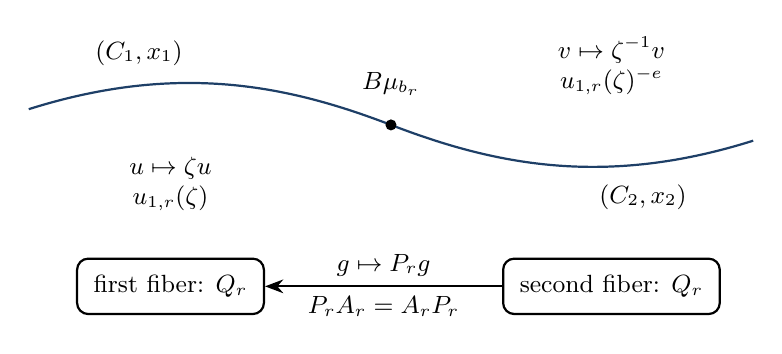
\begin{tikzpicture}[>=Stealth,thick,font=\small]
  \coordinate (n) at (0,0);
  \draw[linkblue] (-4.6,0.2) .. controls (-2.7,0.8) and (-1.3,0.5) .. (n);
  \draw[linkblue] (n) .. controls (1.3,-0.5) and (2.7,-0.8) .. (4.6,-0.2);
  \fill (n) circle (2pt);
  \node[above=5pt] at (-3.2,0.45) {$(C_1,x_1)$};
  \node[below=5pt] at (3.2,-0.45) {$(C_2,x_2)$};
  \node[above=7pt] at (n) {$B\mu_{b_r}$};
  \node[align=center] at (-2.8,-0.75)
    {$u\mapsto\zeta u$\\$u_{1,r}(\zeta)$};
  \node[align=center] at (2.8,0.75)
    {$v\mapsto\zeta^{-1}v$\\$u_{1,r}(\zeta)^{-e}$};
  \node[draw,rounded corners,inner sep=6pt] (f1) at (-2.8,-2.05)
    {first fiber: $Q_r$};
  \node[draw,rounded corners,inner sep=6pt] (f2) at (2.8,-2.05)
    {second fiber: $Q_r$};
  \draw[->] (f2.west) -- node[above] {$g\mapsto P_rg$}
    node[below] {$P_rA_r=A_rP_r$} (f1.east);
\end{tikzpicture}
\caption{The two branches of the balanced node and the torsor fibers on
its normalization, shown schematically.  The cover $w^e=t$ multiplies
boundary monodromy by $e$, and the second branch reverses its orientation.  Multiplication
by $P_r$ identifies the resulting action $u_{1,r}^{-e}$ with
$u_{1,r}$ while commuting with the common Frobenius value $A_r$.}
\label{fig:node-gluing}
\end{figure}


The normalization torsors now glue to a finite \'etale right
$Q_r$-torsor $\mathcal T_{r,0}$ on $\mathcal C(b_r)_0$.  This is
ordinary nodal gluing in the equivariant chart: \'etale locally on
each branch cover, the torsor is constant across the origin; its
two constant fibers have been identified with the same
$\mu_{b_r}$-action.  Glue them across $uv=0$ and take the
equivariant quotient.  This proves \'etaleness at the node as well
as away from it, and retains the $Q_r$-action and semilinear action.
It is the finite-cover gluing of \cite[Section~8.3]{CT}, with the
identification now chosen to commute with $A$.

Proper henselian invariance lifts $\mathcal T_{r,0}$ to a finite
\'etale torsor $\mathcal T_r$ on $\mathcal C(b_r)$
\cite[Theorem~4.5]{Rydh}.  Full faithfulness lifts the group actions,
the equivariance isomorphisms, and the transition maps after pullback
to divisible indices.  Their relations lift as well.  Restriction
to the common geometric generic curve $C$ yields a tower of finite
$Q_r$-torsors and hence, after compatible framing, a continuous
parameter with image in
$\varprojlim_r Q_r=J$.  The lifted equivariance gives the asserted
action on this parameter.

We verify density using the first component, without imposing
connectedness on these $Q_r$-torsors.  Choose a section of
$\mathcal V\to S_{b_*}$ through a point of $(U_1)_{\Dbar}$,
base-change it to every $S_{b_r}$, and choose compatible frames of the
lifted tower along these sections.  Apply
Lemma~\ref{lem:component-orbits} over each $S_{b_r}$.  The orbit of
the frame under the monodromy of the punctured first component lies
in its connected component in the whole special torsor.  The lemma
identifies that component's section fiber with the geometric generic
component's section fiber, which is the generic monodromy orbit.
Thus, if $H_1$ is the image of $\sigma_1$ and $H_\tau$ the image of
$\tau$ in these compatible frames, then
\[
        \operatorname{im}(H_1\to Q_r)
          \subset\operatorname{im}(H_\tau\to Q_r)
        \qquad\text{for every }r.
\]
Both subgroups are compact and therefore closed in $J$.  Since the
$J_r$ are cofinal, these inclusions imply $H_1\subset H_\tau$.
Proposition~\ref{prop:lifted-parameter} makes $H_1$ Zariski dense,
and hence $\tau$ is Zariski dense.

Finally let $V$ be an algebraic representation over a finite
coefficient extension and choose a $J$-stable lattice in $V$.
Every finite reduction factors through some $Q_r$.  Away from the
node the models $\mathcal C(b_r)$ agree with the corresponding
base changes of $\mathcal C(b_*)$.  The torsor $\mathcal T_r$
therefore supplies the required lisse extension on
$\mathcal V\times_{S_{b_*}}S_{b_r}$, and its special restrictions
are exactly the two component torsors with their semilinear actions.
Using this one tower for all representations supplies the tensor and
morphism comparisons, as in Proposition~\ref{prop:lifted-parameter}.
These are the equivariant lattice-specialization data needed for
nearby cycles on the fixed model $\mathcal C(b_*)$.
\end{proof}

\section{From the separating node to an equivariant flag eigensheaf}
\label{sec:nodal}

The parameter $\tau$ of Proposition~\ref{prop:nodal-parameter} lives on
the smooth projective generic curve $C/\Omega$ of the twisted
degeneration.  Proposition~\ref{prop:equivariant-unramified} therefore
supplies an equivariant unramified eigencomplex.  We now specialize
this complex to the node, retain the first normalization component,
and remove the enhancement of its flag.  The two issues are
nonvanishing on the prescribed node type and preservation of the
semilinear action when passing to a perverse eigensheaf.

\begin{proposition}\label{prop:charzero-equivariant}
Let $(C_1,x_1)/D$, $\sigma_1$, and $\varphi$ be the pointed curve,
dense lifted parameter, and semilinear automorphism of
Proposition~\ref{prop:lifted-parameter}.  There exist an integer
$m\geq 1$ and a nonzero locally constructible perverse geometric
$\E$-adic sheaf
\[
 M_{\Dbar}\quad\text{on}\quad
 \mathcal A_1=\Bun_{G,B,x_1}((C_1)_{\Dbar})
\]
with a $\varphi^m$-structure and the full coherent Hecke eigenstructure
for $\sigma_1$.  Every eigenisomorphism is compatible with this
structure and with the given $\varphi^m$-structure on $\sigma_1$.
Moreover, $\SS(M_{\Dbar})\subset\Lambda_{\mathrm{par}}$.
\end{proposition}

\subsection{The prescribed node type and its two flags}

Retain the fixed index $b_*$ and strictly dominant cocharacter
$\lambda$ from Section~\ref{sec:parameters}; thus
\[
 0<\langle\alpha,\lambda\rangle<b_*
 \qquad\text{for every positive root }\alpha.
\]
Put $S=S_{b_*}=\Spec\Dbar[[s_{b_*}]]$.  In the relative bundle stack
of $\mathcal C(b_*)/S$, remove from the closed fiber every inertia
type except the conjugacy class of $\lambda|_{\mu_{b_*}}$.  Denote
the resulting open stack by $\mathcal B$.  The condition is open
because the finitely many conjugacy classes of homomorphisms
$\mu_{b_*}\to G$ are locally constant on the residual gerbe.
The centralizer of the chosen type is $T$: the inequalities ensure
that no root is trivial on $\lambda(\mu_{b_*})$.
The Hom-stack theorem gives algebraicity and local finite
presentation \cite[Theorem~1.2]{HallRydh}.  Smoothness follows from
the vanishing of $H^2$ of the adjoint bundle: the curve is tame,
coarse pushforward is exact, and its coarse space has dimension one.
In particular $\mathcal B$ has smooth finite-type charts over $S$.
Its geometric generic fiber is $\Bun_G(C)$.

Let $B^-$ be the Borel opposite to $B$ with the same maximal torus
$T$, and define
\[
 \mathcal A_1^+=\Bun_{G,R_u(B),x_1}((C_1)_{\Dbar}),
 \qquad
 \mathcal A_2^+=\Bun_{G,R_u(B^-),x_2}((C_2)_{\Dbar}).
\]
An object of either stack includes an enhanced flag, that is, a
reduction to the indicated unipotent radical.  The calculation of
\cite[Lemma~8.2]{CT} gives
\begin{equation}\label{eq:nodal-type-quotient}
 \mathcal B_s\simeq
       [\mathcal A_1^+\times\mathcal A_2^+/T],
\end{equation}
where $T$ changes the two frames on the node gerbe simultaneously.
We recall the calculation to verify its compatibility with our
semilinear action and with the two different component curves.

On the first branch of the balanced chart, set $a=u^{b_*}$.
In a frame in which inertia is $\lambda$, a change of frame satisfies
\[
 h(\zeta u)=\lambda(\zeta)h(u)\lambda(\zeta)^{-1}.
\]
Conjugating to the invariant punctured-disc frame gives
$g(a)=\lambda(u)^{-1}h(u)\lambda(u)$.  If
$j=\langle\alpha,\lambda\rangle$ for a positive root, the positive
and negative root coordinates respectively transform as
\begin{equation}\label{eq:nodal-root-coordinate}
 u^j f(u^{b_*})\longmapsto f(a),
 \qquad
 u^{b_*-j}g(u^{b_*})\longmapsto a g(a).
\end{equation}
The toral coordinates are series in $a$.  These formulas identify
the full frame-change group with
$\{g(a)\in G(\Dbar[[a]]):g(0)\in B\}$; the assertion over arbitrary
test schemes follows by the same root-group factorization in the
formal big cell.  Evaluation $h\mapsto h(0)$ becomes the torus
projection of this Iwahori group.  Fixing the gerbe frame therefore
gives an enhanced $B$-flag.

On the second branch the node generator acts by
$v\mapsto\zeta^{-1}v$.  Its positively oriented coordinate generator
thus sees $-\lambda$, so the identical calculation gives $B^-$.
On both branches the fixed gerbe torsor has automorphism group $T$,
expressed using the common node generator.  Gluing the normalization bundles, with an
identification on their gerbes, now gives
\eqref{eq:nodal-type-quotient}.  The computation is branchwise and
requires no isomorphism between $C_1$ and $C_2$.

All these prescriptions use the split group, the group-scheme
cocharacter $\lambda$, and the balanced coordinates chosen over
$D$.  They consequently commute with $\varphi$, including its
action on $\mu_{b_*}$; no individual root of unity has been declared
fixed.  Thus \eqref{eq:nodal-type-quotient} is an equivariant
identification.  A modification away from the node preserves its
gerbe frames and acts on the corresponding factor.  This also
identifies every successive and multi-leg Hecke correspondence,
after pullback to $\mathcal A_1^+\times\mathcal A_2^+$, with its
componentwise counterpart.

\subsection{A criterion for nonzero nearby cycles}

Nearby cycles can vanish for a nonzero generic complex.  The input
that excludes this possibility here is the specialization-detection
theorem of \cite[Theorem~4.2]{CT}, with the following precise scope.

\begin{lemma}[Specialization detection]\label{lem:specialization-detection}
Let $S=\Spec A$ be an excellent complete strictly henselian trait
with algebraically closed residue field and $\ell$ invertible.
Let $\mathcal Y\to S$ be smooth and locally of finite type.  Its
special fiber is to be an unlevelled, ordinary Borel-level, or
enhanced Borel-level bundle stack on a smooth projective curve, or,
in characteristic zero, the simultaneous-torus quotient of two
enhanced-level stacks.  If the residue characteristic is positive,
assume that the residue field is an algebraic closure of a finite
field and impose the Lie-theoretic hypotheses of
Lemma~\ref{lem:lie-hypotheses}.

Assume that a smooth scheme $L\to S$ of relative dimension one
provides spherical Hecke legs and that $L_s$ contains a nonempty
open of each special-fiber curve on which modifications are allowed.
The bounded output maps to $\mathcal Y\times_S L$ must be
representable and proper; exact-relative-position strata must be
smooth over both input-and-leg and output-and-leg; their special
fibers must have the transverse-modification geometry of
\cite[Proposition~3.3]{CT}.  The Satake kernel on its open stratum is
constant with the relative Satake shift and twist.

Let $F$ be a locally bounded constructible complex on
$\mathcal Y_{\bar\eta}$ with lisse spherical Hecke eigenvalues on
$L_{\bar\eta}$.  Suppose each eigenvalue has a lisse lattice whose
finite reductions extend lisse after finite trait extensions,
compatibly with the special-fiber value, as in
Proposition~\ref{prop:equivariant-specialization}.
If, on some smooth finite-type chart $Z\to\mathcal Y$, the closure
of the nonzero-stalk locus of $F|_{Z_{\bar\eta}}$ meets $Z_s$, then
$\Psi F\ne0$.
\end{lemma}

Here and below $\Psi$ is geometric nearby cycles, without inertia
invariants.  The closure in the lemma may be computed after
descending its finitely many geometric generic components to a
finite extension of the trait.  Neither the lemma nor this
interpretation requires the complex $F$ itself to descend.
These are part of the statement and conventions of
\cite[Theorem~4.2]{CT}.

We will produce the required meeting by extending a bundle carrying
a nonzero generic stalk.  For $G=\SL_n$, the uniformization needed
for this step has an elementary description.  If $Y$ is a smooth
projective connected curve over an algebraically closed field and
$y\in Y$, the complement $Y\setminus\{y\}$ is a smooth affine curve.
Its coordinate ring is a Dedekind domain.  A rank-$n$ projective
module over that ring is isomorphic to the sum of a free module of
rank $n-1$ and its determinant.  Consequently every $\SL_n$-bundle
is trivial on this complement.  A free basis can be adjusted by a
unit so that its determinant agrees with the given trivialization.
This is the $\SL_n$ case of the affine-curve triviality used in
Drinfeld--Simpson uniformization and in
\cite[Theorem~1.1]{BelkaleFakhruddin}; see also
\cite{DrinfeldSimpson}.

In particular, any two $\SL_n$-bundles on $Y$ differ by a
modification at $y$.  Each such modification lies in some finite
Schubert bound.  In a family, the bounded Hecke space with fixed
reference input and fixed smooth section $y$ is proper over the
base trait.  A geometric generic modification therefore extends
after a finite trait extension: its point first descends to a
finite generic extension, and the valuative criterion then applies
over the corresponding DVR normalization of the complete trait.
The output remains unchanged near every
marking or node disjoint from $y$.

\subsection{Specializing on the chosen component}

Apply Proposition~\ref{prop:equivariant-unramified} to $(C,\tau)$.
The generic curve is smooth, projective, and connected of genus at
least two; its polarization comes from the projective smoothing.
Proposition~\ref{prop:nodal-parameter} supplies the continuous dense
parameter over a finite coefficient field and its equivariance.
We obtain a nonzero locally bounded constructible eigencomplex
$D_\tau$ on $\mathcal B_{\bar\eta}=\Bun_G(C)$, with its
$\varphi$-structure and coherent equivariant eigenmaps.

The trait $S_{b_*}$ is excellent, complete, and strictly henselian,
with algebraically closed characteristic-zero residue field; in
particular $\ell$ is invertible.  Use $L=\mathcal V$, the smooth
scheme locus of $\mathcal C(b_*)$, a relative curve with
$L_{\bar\eta}=C$ and $L_s=U_{1,\Dbar}\sqcup U_{2,\Dbar}$.
At these legs the bounded correspondences have the split affine
Grassmannian models in smooth frame charts.  Their output maps are
representable and proper, and their exact-position maps are smooth
over both bundle-and-leg projections.  These local models have the
normalized constant kernels on their open cells.  Modifications
there preserve the node type.  On the special fiber
\eqref{eq:nodal-type-quotient}, the cotangent description, cone
dimension bound, and transverse modifications are precisely the
torus-quotient case of \cite[Section~3 and Section~8.2]{CT}.
The required Lie-theoretic properties hold in characteristic zero.
Thus the geometric hypotheses of
Proposition~\ref{prop:equivariant-specialization} and
Lemma~\ref{lem:specialization-detection} hold for this family.

For their eigenvalue hypothesis, use the equivariant finite-torsor
tower of Proposition~\ref{prop:nodal-parameter}.  For each
representation, an invariant lattice has reductions extending
lisse over the smooth scheme locus after the extensions
$S_{b_r}\to S_{b_*}$.  Their specializations are the component
parameter systems, and all tensor maps and semilinear actions are
carried by the same tower.  Hence
\begin{equation}\label{eq:nodal-nearby}
 F_s:=\Psi D_\tau
\end{equation}
is locally bounded constructible and carries the coherent component
eigenstructure and its $\varphi$-action.

To prove $F_s\ne0$ on this particular type, first choose a point of
$\mathcal A_1^+\times\mathcal A_2^+$.  A smooth chart of
$\mathcal B$ through its image, followed by henselian lifting,
gives a reference bundle $P_0$ over $S$ with the prescribed node
type.  Lift also a point of $L_s$ to a section $y$ of $L/S$.
Choose a bundle $P$ on $C/\Omega$ where $D_\tau$ has nonzero stalk.
Such a point exists on a finite-type chart because $D_\tau$ is
nonzero and locally bounded constructible.

The Dedekind-domain argument above identifies $P$ and $(P_0)_\Omega$
off $y_\Omega$.  Extend the resulting bounded modification after a
finite trait extension.  Its output lies in $\mathcal B$, since its
node restriction still equals that of $P_0$.  Take a smooth
finite-type chart $Z\to\mathcal B$ through its special value and a
residue-field point of the chart above it.  If $S'$ is the extended
trait, the morphism $Z\times_{\mathcal B}S'\to S'$ is smooth;
henselian lifting of that point gives a section, after a further
finite extension if necessary.  Its geometric generic
point has the chosen nonzero stalk.  This section witnesses a
meeting of the closure in Lemma~\ref{lem:specialization-detection}
with the special fiber.  Thus
\begin{equation}\label{eq:nodal-nonzero}
 F_s\ne0\quad\text{on }[\mathcal A_1^+\times\mathcal A_2^+/T].
\end{equation}
Finite extensions in this argument only locate the closure inside
the fixed geometric generic fiber; they impose no new descent
condition on $D_\tau$ or its semilinear structure.  They need not
carry $\varphi$: geometric nearby cycles are unchanged by this
finite-trait replacement, and the equivariant object
\eqref{eq:nodal-nearby} was already constructed over $S$.

Ordinary pullback of $F_s$ to
$\mathcal A_1^+\times\mathcal A_2^+$ is nonzero, because this map is
smooth and surjective.  Choose a $\Dbar$-point $(a_1,a_2)$ with
nonzero stalk.  The bundle and enhanced flag defining $a_2$ descend
to a finite extension $D'/D$: they are of finite presentation and
$\Dbar/D$ is algebraic.  Pass to a finite normal extension
containing $D'$.  Since $\varphi$ fixes $D$, its action on this
normal extension has finite order.  Some power $\varphi^m$ fixes
it pointwise, and the descended model then supplies an
identification $\varphi^{m*}a_2\simeq a_2$.  We henceforth use this
power as generator.

Restricting along $\mathcal A_1^+\times\{a_2\}$ gives a nonzero
locally bounded constructible complex $F_1^+$ on $\mathcal A_1^+$,
with a $\varphi^m$-structure.  The quotient description of the Hecke
correspondences and proper base change for each bound give
\begin{equation}\label{eq:nodal-enhanced-eigen}
 \Hecke_{I,(V_i)}(F_1^+)
   \simeq F_1^+\boxtimes
                 \mathop{\boxtimes}_{i\in I}(V_i)_{\sigma_1}
\end{equation}
for every finite leg set $I$.  The same comparisons apply on the
successive-modification spaces and on every fusion diagonal.
They are natural under semilinear transport, so all these
eigenmaps and their coherence constraints are equivariant.
Ordinary restriction here is sufficient; no perversity assertion
is made for $F_1^+$.

\subsection{Perverse cohomology and removal of the enhancement}

To pass from $F_1^+$ to an ordinary-level perverse eigensheaf, we
will take perverse cohomology, push forward along the torsor that
forgets the enhancement, and take perverse cohomology once more.
The first truncation supplies nilpotent singular support, which
controls monodromy along the enhancement torus.  Unipotence of that
monodromy will ensure that the direct image is nonzero; the second
truncation then gives the required perverse object.

The geometric inputs for these steps are
\cite[Propositions~6.1 and 7.5]{CT}.  Their scope is a smooth
projective complex curve with one marked
point and a split simple simply connected group.  Proposition~6.1
applies at either ordinary or enhanced Borel level: for a locally
bounded constructible geometric adic complex with a coherent
eigenstructure for a Zariski-dense parameter, every perverse
cohomology inherits the full eigenstructure and nilpotent singular
support, and some perverse cohomology is nonzero if the complex is.
Proposition~7.5 removes the enhancement when the boundary monodromy
is unipotent.  Our group $\SL_n$ meets the group assumptions, and
Proposition~\ref{prop:lifted-parameter} proves both density and the
required unipotent boundary monodromy for $\sigma_1$.

Choose an abstract field isomorphism $\Dbar\simeq\C$ to apply these
geometric statements.  Such an isomorphism exists: both fields
are algebraically closed of characteristic zero and have
transcendence degree $2^{\aleph_0}$ over $\Q$.  We will use their
Betti arguments to establish geometric properties, while making
all sheaf operations and induced maps in the geometric adic
category over $\Dbar$.

First choose $j$ such that $Q={}^pH^j(F_1^+)\ne0$.
Here is why its eigenstructure retains the semilinear action.
For a finite set $I$, put $d=|I|$.  The proof of
\cite[Proposition~6.1, Section~6.3]{CT} constructs, on the objects
under consideration, the functorial adic comparison
\begin{equation}\label{eq:nodal-truncation}
 {}^pH^j\bigl(\Hecke_{I,(V_i)}(F_1^+)[d]\bigr)
 \simeq \Hecke_{I,(V_i)}({}^pH^jF_1^+)[d].
\end{equation}
The Betti calculation proves the needed perverse bounds; the
comparison itself follows from the universal property of the
adic truncation triangles.  On the eigenvalue side, put
$\mathcal L_I=\boxtimes_{i\in I}(V_i)_{\sigma_1}$.  Since this
sheaf is lisse on the smooth $d$-dimensional leg space, exterior
product with $\mathcal L_I[d]$ is perverse exact, so
\[
 {}^pH^j(F_1^+\boxtimes\mathcal L_I[d])
       \simeq Q\boxtimes\mathcal L_I[d].
\]
Applying these comparisons to \eqref{eq:nodal-enhanced-eigen}
and canceling the common shift $[d]$ gives the relative-normalized
eigenmaps for $Q$.

For a collision $\Delta:U_1^J\to U_1^I$, the corresponding
truncation comparison uses
$(\id\times\Delta)^*[|J|-|I|]$ on these locally constant leg
families.  The comparisons for successive Hecke operations use the
total dimension of their retained leg space, counting a shared
leg only once.  Thus \eqref{eq:nodal-truncation} carries the entire
unit, convolution, permutation, and fusion diagrams.  Pullback by
$\varphi^m$ preserves the perverse structure and its truncation
maps, so these adic comparisons commute with it.  No compatibility
between a chosen complex realization and $\varphi$ is needed.

Now let
\[
 q:\mathcal A_1^+\longrightarrow\mathcal A_1
\]
forget the enhancement.  This is a $T$-torsor of relative dimension
$r=n-1$.  Set $F=q_!Q$.  We need the intermediate assertion in the
proof of \cite[Proposition~7.5]{CT}: this particular direct image is
nonzero.  We recall its mechanism, since a general torus direct
image does not preserve nonvanishing.

At enhanced level, a cotangent residue lies in $\operatorname{Lie}B$.
In an adapted local frame write a generically nilpotent Higgs field
as $\theta=b(t)\,dt/t$, with $b(t)$ regular.  The positive-degree
invariant polynomials vanish on $b(t)$ and hence on the residue
$b(0)$; the toral projection of this residue is therefore zero.
Thus the enhanced nilpotent cone is the smooth cotangent pullback
of the ordinary-level cone and annihilates tangent directions to
the $T$-fibers \cite[Section~3.1]{CT}.  The microlocal criterion of
\cite[Lemma~7.1]{CT} now makes the Betti realization of $Q$
monodromic along this torsor: locally on the base it is constructible
for a product stratification with the whole torus as second factor.
In particular its cohomology sheaves on each fiber are local systems.

For a representation $V$, let $\chi_V$ be its character on the
dual torus $\widehat T$.  The central-sheaf calculation, based on
Gaitsgory's construction \cite{GaitsgoryCentral} and proved in the
needed form in \cite[Lemma~7.4 and proof of Proposition~7.5]{CT},
gives, for
every $V\in\Rep(\Gd)$,
\begin{equation}\label{eq:nodal-character}
 \chi_V(\text{enhancement monodromy})
       =\operatorname{Tr}(\text{boundary monodromy on }V_{\sigma_1})
          \,\id_Q
       = (\dim V)\,\id_Q.
\end{equation}
The last equality uses unipotence at $x_1$.  On any stalk
cohomology of a torsor fiber, the commuting monodromies have joint
generalized eigencharacters, viewed as points of the dual torus
$\widehat T(\E)$.  Character functions of representations span the
Weyl-invariant regular functions on $\widehat T$ and separate its
Weyl orbits.  Equation
\eqref{eq:nodal-character} therefore puts each eigencharacter in
the orbit of $1$, which consists of $1$ alone.  All enhancement
monodromies on these finite-dimensional spaces are unipotent.

Choose a fiber $T=q^{-1}(a)$ where $Q_T:=Q|_T$ is nonzero, and let
$j_0$ be the largest index with $\mathcal H^{j_0}(Q_T)\ne0$.
Its fiber $W$ is a nonzero finite-dimensional representation of
$\Gamma=X_*(T)$ with commuting unipotent operators.  The
augmentation ideal of $\E[\Gamma]$ acts nilpotently on this space,
so the coinvariants $W_\Gamma$ are nonzero.  Poincar\'e duality gives
\[
 H_c^{2r}(T,\mathcal H^{j_0}(Q_T))
       \simeq W_\Gamma(-r)\ne0.
\]
In the compact-support hypercohomology spectral sequence this term
has no incoming differential, by maximality of $j_0$, and no
outgoing differential, because $H_c^i(T,-)=0$ for $i>2r$.
Consequently $H_c^{2r+j_0}(T,Q_T)\ne0$.  Comparison and base change
for the adic functor $q_!$ imply $F_a\ne0$.  This argument uses a
nilpotence bound only on the chosen finite-dimensional space.

The morphism $q$ has finite type and fixed relative dimension, so
$F$ is locally bounded constructible.  Away from $x_1$, Hecke
modifications transport an enhanced flag as well as its ordinary
flag.  Proper base change on a bounded Hecke correspondence and
the projection formula therefore give the natural comparison
\begin{equation}\label{eq:nodal-torus-hecke}
 \Hecke_{I,(V_i)}(q_!Q)
 \simeq (q\times\id_{U_1^I})_!\Hecke_{I,(V_i)}(Q)
 \simeq q_!Q\boxtimes
                  \mathop{\boxtimes}_{i\in I}(V_i)_{\sigma_1}.
\end{equation}
These comparisons also hold on the successive and collision
correspondences.  Hence they preserve every coherence constraint.
Since $q$ is defined over $D$, its direct image and these natural
comparison maps carry the $\varphi^m$-structure.

Finally choose a nonzero perverse cohomology
$M_{\Dbar}={}^pH^a(F)$.  Proposition~6.1 of \cite{CT} applies now
at ordinary Borel level, and the same adic truncation argument
\eqref{eq:nodal-truncation} proves equivariance of all the induced
eigenmaps.  It also gives nilpotent singular support.  At ordinary
flag level this is $\Lambda_{\mathrm{par}}$.
This completes the proof of Proposition~\ref{prop:charzero-equivariant}.

\section{Specialization to the finite field}
\label{sec:final}

We now have a perverse eigensheaf with an action of $\varphi^m$ on
the lifted pointed curve over $\Dbar$.  The arithmetic torsor tower
of Proposition~\ref{prop:lifted-parameter} identifies its eigenvalue
after mixed-characteristic specialization with the original
arithmetic parameter, including its Frobenius structure.

\begin{proof}[Proof of Theorem~\ref{thm:main}]
Take $m$ and $M_{\Dbar}$ from
Proposition~\ref{prop:charzero-equivariant}.  Recall that
$R=W(k)$, $K=\overline{\Frac(R)}$, and $\Dbar\subset K$ is
preserved by $\varphi$.  Pullback under this algebraically closed
field extension gives
\[
 M_K\quad\text{on}\quad
 \Bun_{G,B,\mathfrak x}(\mathscr X_K).
\]
It remains nonzero, locally constructible, and perverse, and
inherits the $\varphi^m$-structure.  These assertions are checked
on finite-type smooth charts: extension of algebraically closed
fields preserves nonzero constructible stalks, support dimensions,
and Verdier duality, hence perversity.  Base change for the bounded
Hecke correspondences, with the tensor Satake comparison of
Section~\ref{sec:conventions}, transports the entire eigenstructure.
Its eigenvalue is the base change of $\sigma_1$, with the action
provided by the arithmetic tower.

Consider the relative ordinary-level bundle stack
\begin{equation}\label{eq:final-relative-stack}
 \mathscr A=
 \Bun_{G,B,\mathfrak x}(\mathscr X_R/R),
 \qquad L=\mathscr U_R,
 \qquad M=\Psi M_K\quad\text{on }\mathscr A_k.
\end{equation}
We verify the hypotheses of
Proposition~\ref{prop:equivariant-specialization} and
Lemma~\ref{lem:specialization-detection} in this second family.
The ring $R$ is an excellent complete strictly henselian DVR with
algebraically closed residue field $k$, and $\ell$ is invertible
because $\ell\ne p$.  The stack $\mathscr A$ is smooth and locally
of finite type over $R$: $H^2$ of the adjoint bundle vanishes on
the fibers of the smooth relative curve, and adding a flag is a
smooth $G/B$-fibration.  The leg space $L$ is smooth of relative
dimension one, with special fiber $U$.

Since all legs avoid $\mathfrak x$, their spherical Hecke
correspondences have the ordinary split affine Grassmannian
models in frames.  Bounded output maps are representable and
proper, both exact-position maps over bundle-and-leg are smooth,
and the open-stratum kernels have the fixed relative Satake
normalization.  The special-fiber cotangent and
transverse-modification geometry is the ordinary Borel-level
case of \cite[Section~3]{CT}.  Its group hypotheses H1--H4 hold
by Lemma~\ref{lem:lie-hypotheses}, using $p>n$.
Finally, the invariant lattices supplied by the arithmetic tower
have lisse finite reductions on $\mathscr U_R$, with their
$\varphi$-actions.  Their specializations, including all tensor
maps, are exactly the local systems associated to $\rho$.
Thus all the geometric and eigenvalue hypotheses of both cited
specialization statements hold.

It follows that $M$ is locally constructible and perverse, and
has the natural multi-leg eigenisomorphisms
\begin{equation}\label{eq:final-eigen}
 \Hecke_{I,(V_i)}(M)
 \simeq M\boxtimes
                 \mathop{\boxtimes}_{i\in I}(V_i)_{\rho|_{\pi_1(U)}}.
\end{equation}
The same proposition gives a $\varphi^m$-structure on $M$ and
equivariance of these maps.  The special-fiber action of
$\varphi^m$ is $q^m$-Frobenius.  On the eigenvalue system its
action is precisely the one obtained by restricting
$\rho$ to $\pi_1(U_{0,\F_{q^m}})$, because the finite torsors used
for the lift descended from that arithmetic representation.
This identifies the arithmetic eigenvalue, as well as its
geometric restriction.

We still have to prove $M\ne0$.  Choose a $K$-point $(P,\beta)$
with nonzero stalk of $M_K$, where $\beta$ is its Borel reduction
at $\mathfrak x_K$.  Use the trivial $G$-bundle on $\mathscr X_R$
as reference, and lift a point of $U(k)$ to a section
$y\in\mathscr U_R(R)$ by smoothness and the henselian property.
The affine-curve argument of Section~\ref{sec:nodal} trivializes
$P$ off $y_K$, compatibly with its determinant.  The resulting
modification of the reference bundle lies in a finite Schubert
bound, whose Hecke space is proper over the reference input and
$y$.  After a finite trait extension it extends to a bundle
$\mathscr P$ on the whole relative curve.

The remaining datum is the flag.  Its generic value $\beta$ is a
point of the associated flag bundle
$\mathscr P|_{\mathfrak x}\times^G G/B$ over the extended trait.
This bundle is proper, so the valuative criterion extends
$\beta$ as well.  We have thereby extended the point
$(P,\beta)$ to a section of $\mathscr A$.  Lift this section to a
smooth finite-type chart through its special value, using
henselian lifting as in the nodal argument.  The section has a
nonzero generic stalk, so the closure of the nonzero-stalk locus
on that chart meets its special fiber.  All hypotheses having
been verified above, Lemma~\ref{lem:specialization-detection}
proves $M\ne0$.

Apply now the field-level nilpotent-detection theorem
\cite[Theorem~4.1]{CT}.  For the level stacks over
$k=\overline{\F}_q$ under its Lie-theoretic hypotheses, it states
that a locally bounded constructible
complex with spherical eigenisomorphisms and lisse eigenvalues
has singular support in the cone of generically nilpotent Higgs
fields on every smooth finite-type chart.  Here $\mathscr A_k$
is the ordinary Borel-level stack, the characteristic assumptions
hold, and \eqref{eq:final-eigen} supplies those lisse eigenvalues.
At an ordinary flag $\beta$, the cotangent residue condition is
\[
 \operatorname{Res}_{x}\theta
        \in\operatorname{Lie}R_u(B_\beta).
\]
The cone in the detection theorem is therefore exactly
$\Lambda_{\mathrm{par}}$ from Theorem~\ref{thm:main}.  This proves
$\SS(M)\subset\Lambda_{\mathrm{par}}$ in the stated chartwise sense.

Equip $M$ with its $\varphi^m$-structure and denote the resulting
Weil sheaf over $\F_{q^m}$ by $M_0$.  The split Weil Satake
comparison of Section~\ref{sec:conventions} identifies the
transported Hecke functors with the relative-Satake-normalized
Weil functors in the theorem.  Thus \eqref{eq:final-eigen} is an
isomorphism of Weil sheaves for every finite leg set and every
collection of representations.

Every operation above transports the full eigenstructure by
comparisons natural for the semilinear generator.  These
comparisons were constructed on the successive-modification
correspondences and on every collision diagonal, with the tensor
unit and permutations respected throughout.  The resulting
unit, convolution, permutation, and fusion diagrams therefore
commute as Weil diagrams, including all iterated collisions.
A structure for the group generated by Frobenius is all that is
required for a Weil sheaf; no profinite descent assertion is
used.  The resulting $M_0$ has all the claimed properties.
\end{proof}

\begin{thebibliography}{AGKRRV}

\bibitem[AV]{AbramovichVistoli}
D.~Abramovich and A.~Vistoli, \emph{Compactifying the space of stable maps},
J. Amer. Math. Soc. \textbf{15} (2002), no.~1, 27--75.

\bibitem[AGKRRV]{AGKRRV}
D.~Arinkin, D.~Gaitsgory, D.~Kazhdan, S.~Raskin, N.~Rozenblyum, and
Y.~Varshavsky, \emph{The stack of local systems with restricted variation
and geometric Langlands theory with nilpotent singular support},
arXiv:2010.01906v2, April 6, 2022.

\bibitem[Bar]{Barrett}
O.~Barrett, \emph{The singular support of an $\ell$-adic sheaf},
Tunisian J. Math. \textbf{6} (2024), no.~4, 703--734.

\bibitem[Bei]{Beilinson}
A.~Beilinson, \emph{Constructible sheaves are holonomic},
Selecta Math. (N.S.) \textbf{22} (2016), no.~4, 1797--1819.

\bibitem[BBD]{BBD}
A.~A.~Beilinson, J.~Bernstein, and P.~Deligne, \emph{Faisceaux pervers},
in \emph{Analyse et topologie sur les espaces singuliers~I},
Ast\'erisque \textbf{100} (1982), 5--171.

\bibitem[BF]{BelkaleFakhruddin}
P.~Belkale and N.~Fakhruddin, \emph{Triviality properties of principal
bundles on singular curves}, Algebraic Geometry \textbf{6} (2019),
no.~2, 234--259.

\bibitem[Dri]{Drinfeld}
V.~G.~Drinfeld, \emph{Two-dimensional $\ell$-adic representations of
the fundamental group of a curve over a finite field and automorphic
forms on $\mathrm{GL}(2)$}, Amer. J. Math. \textbf{105} (1983), no.~1,
85--114.

\bibitem[DS]{DrinfeldSimpson}
V.~G.~Drinfeld and C.~Simpson, \emph{$B$-structures on $G$-bundles and
local triviality}, Math. Res. Lett. \textbf{2} (1995), no.~6, 823--829.

\bibitem[F\ae r]{Faergeman}
J.~F\ae rgeman, \emph{Motivic realization of rigid $G$-local systems on
curves and tamely ramified geometric Langlands},
arXiv:2405.18268v2, July 28, 2024; to appear in Selecta Mathematica.

\bibitem[FGV]{FGV}
E.~Frenkel, D.~Gaitsgory, and K.~Vilonen, \emph{On the geometric
Langlands conjecture}, J. Amer. Math. Soc. \textbf{15} (2002), no.~2,
367--417.

\bibitem[Gai01]{GaitsgoryCentral}
D.~Gaitsgory, \emph{Construction of central elements in the affine
Hecke algebra via nearby cycles}, Invent. Math. \textbf{144} (2001),
no.~2, 253--280.

\bibitem[Gai04]{GaitsgoryVanishing}
D.~Gaitsgory, \emph{On a vanishing conjecture appearing in the geometric
Langlands correspondence}, Ann. of Math. (2) \textbf{160} (2004),
no.~2, 617--682.

\bibitem[GKRV]{GKRV}
D.~Gaitsgory, D.~Kazhdan, N.~Rozenblyum, and Y.~Varshavsky,
\emph{A toy model for the Drinfeld--Lafforgue shtuka construction},
arXiv:1908.05420v5, February 7, 2022.

\bibitem[GR]{GR}
D.~Gaitsgory and S.~Raskin, \emph{Geometric Langlands in positive
characteristic from characteristic zero}, arXiv:2508.02237v1,
August 4, 2025.

\bibitem[HR]{HallRydh}
J.~Hall and D.~Rydh, \emph{Coherent Tannaka duality and algebraicity of
Hom-stacks}, Algebra Number Theory \textbf{13} (2019), no.~7, 1633--1675.

\bibitem[HS]{HansenScholze}
D.~Hansen and P.~Scholze, \emph{Relative perversity},
Commun. Amer. Math. Soc. \textbf{3} (2023), 631--668.

\bibitem[Lau]{Laumon}
G.~Laumon, \emph{Correspondance de Langlands g\'eom\'etrique pour les
corps de fonctions}, Duke Math. J. \textbf{54} (1987), no.~2, 309--359.

\bibitem[LO]{LieblichOlsson}
M.~Lieblich and M.~Olsson, \emph{Generators and relations for the
\'etale fundamental group}, Pure Appl. Math. Q. \textbf{6} (2010),
no.~1, 209--243.

\bibitem[MV]{MV}
I.~Mirkovi\'c and K.~Vilonen, \emph{Geometric Langlands duality and
representations of algebraic groups over commutative rings},
Ann. of Math. (2) \textbf{166} (2007), no.~1, 95--143;
corrected version arXiv:math/0401222v5, February 13, 2018.

\bibitem[NY]{NYAutomorphicGluing}
D.~Nadler and Z.~Yun, \emph{Automorphic gluing functor in Betti
geometric Langlands}, arXiv:2105.12318v3, June 6, 2023.

\bibitem[Ols]{OlssonTwisted}
M.~C.~Olsson, \emph{(Log) twisted curves}, Compos. Math.
\textbf{143} (2007), no.~2, 476--494.

\bibitem[CT]{CT}
OpenAI, \emph{Constructible tame Hecke eigensheaves in positive
characteristic}, OpenAI Math Release preprint
\href{https://github.com/openai/math/blob/main/preprints/Constructible-tame-Hecke-eigensheaves-in-positive-characteristic-October-5-2026/constructible-tame-hecke-eigensheaves-positive-characteristic.pdf}{OAI:Constructible-tame-Hecke-eigensheaves-in-positive-characteristic-October-5-2026},
2026.

\bibitem[Ryd]{Rydh}
D.~Rydh, \emph{Compactification of stacks and extending stackiness
across the boundary}, preprint, September 16, 2014.

\end{thebibliography}

\end{document}
